
\newif\ifcrossling\crosslingtrue
\newif\ifitmtree\itmtreetrue
\newif\iflong\longfalse
\newif\ifevaluation\evaluationfalse
\newif\ifconjugacy\conjugacyfalse
\newif\ifnonpar\nonparfalse
\newif\ifling\lingfalse
\newif\ifhighlevel\highleveltrue
\newif\iftmreview\tmreviewfalse
\newif\ifevocation\evocationfalse
\newif\ifsupershortmlslda\supershortmlsldatrue

\documentclass[compress]{beamer}

%\usepackage{beamerthemesplit}
\usepackage{xmpmulti}

\definecolor{green}{rgb}{0,.3,0}

\usepackage{graphicx,float,wrapfig, bbm}
\usepackage{amsfonts, bbold, comment}
\usepackage{mdwlist}
\usepackage{listings}
\usepackage{environ}
\usepackage{subfigure}
\usepackage{rotating}
\usepackage{algorithmic}
\usepackage{algorithm}
\usepackage{overpic}

\usepackage{multirow}

\usetheme{Rochester}
%\useoutertheme{infolines}
%\usetheme{Boadilla}
%\usetheme{Singapore}
\usecolortheme{umd}
\title{Big Data Analysis with Topic Models: Human Interaction, Streaming Computation, \\and Social Science Applications}
\author{Jordan Boyd-Graber}
\date{\today}

\newcommand{\fsi}[2]{
\begin{frame}[plain]
\vspace*{-1pt}
\makebox[\linewidth]{\includegraphics[width=\paperwidth]{#1}}
\begin{center}
#2
\end{center}
\end{frame}
}


\newcommand{\explain}[2]{\underbrace{#2}_{\mbox{\footnotesize{#1}}}}
\newcommand{\dir}[1]{\mbox{Dir}(#1)}
\newcommand{\mult}[1]{\mbox{Mult}( #1)}
\newcommand{\Beta}[1]{\mbox{Beta}( #1)}
\newcommand{\G}[1]{\Gamma \left( \textstyle #1 \right)}
\newcommand{\LG}[1]{\log \Gamma \left( \textstyle #1 \right)}
\newcommand{\WN}[0]{\textsc{WordNet}}
\newcommand{\itmspace}[0]{\hspace{2cm}}
\newcommand{\abr}[1]{\textsc{#1}}
\newcommand{\lda}[0]{\abr{lda}}
\newcommand{\slda}[0]{\abr{slda}}

\newcommand{\digam}[1]{\Psi \left( \textstyle #1 \right) }
\newcommand{\ddigam}[1]{\Psi' \left( \textstyle #1 \right) }
\newcommand{\e}[2]{\mathbb{E}_{#1}\left[ #2 \right] }
\newcommand{\ind}[1]{\mathbb{I}\left[ #1 \right] }
\newcommand{\ex}[1]{\mbox{exp}\left\{ #1\right\} }
\newcommand{\D}[2]{\frac{\partial #1}{\partial #2}}
\newcommand{\elbo}{\mathcal{L}}


\newcommand{\citename}[1]{\emph{#1} }
\newcommand{\bm}[1]{\mbox{\boldmath$#1$}}
\newcommand{\Dir}{\mathrm{Dir}}
\newcommand{\Mult}{\mathrm{Mult}}
\newcommand{\g}[1]{\Gamma \left( #1 \right)}
\newcommand{\paragraph}[1]{ \vskip 1cm {\bf \large #1}}

\NewEnviron{smalign}{
\vspace{-.6cm}
\begin{small}
\begin{align}
  \BODY
\end{align}
\end{small}
\vspace{-.6cm}
}


\providecommand{\graphscale}{0.6}

\newcommand{\danquote}[1]{

\begin{flushright}
\begin{overpic}[width=5.5cm,tics=10]{general_figures/speech_bubble}
	\put(10,30) { \parbox{4cm}{#1 }}
\end{overpic}

\includegraphics[width=1.5cm]{general_figures/milkman_dan}
\end{flushright}
}


% \AtBeginSection[] % "Beamer, do the following at the start of every section"
% { \begin{frame}

% \frametitle{Outline} % make a frame titled "Outline"
% \tableofcontents[currentsection] % show TOC and highlight current section
% \end{frame} }

\lstset{language=Python}

\DeclareMathSymbol{\R}{\mathbin}{AMSb}{"52}

%\setbeamertemplate{footline}{\hspace*{.5cm}\scriptsize{\insertauthor

\begin{document}

% this prints title, author etc. info from above

\frame{\titlepage
\vspace{-2cm}

\includegraphics[width=0.3\linewidth]{general_figures/umd_logo} \\
\tiny

}



\begin{frame}
\frametitle{The Challenge of Big Data}

\begin{columns}

\column{.5\linewidth}

Every second \dots
\begin{itemize}
  \item 600 new blog posts appear
  \item 34,000 tweets are tweeted
  \item 30 GB of data uploaded to Facebook
\end{itemize}
\pause

\begin{block}{Unstructured}
  No XML, no semantic web, no annotation.  Often just raw text.
\end{block}

\column{.5\linewidth}

\only<3->{
Common task: what's going on in this dataset.
\begin{itemize}
   \item Intelligence analysts
   \item Brand monitoring
   \item Journalists
   \item Humanists
\end{itemize}
}
\only<4>{
\centering
Common solution: topic models
}

\end{columns}

\end{frame}

\begin{frame}

\begin{center}
\frametitle{Topic Models as a Black Box}
From an \textbf<1>{input corpus} and number of topics \textbf<1>{$K$} $\rightarrow$ \textbf<2>{words to topics} \\
\only<1>{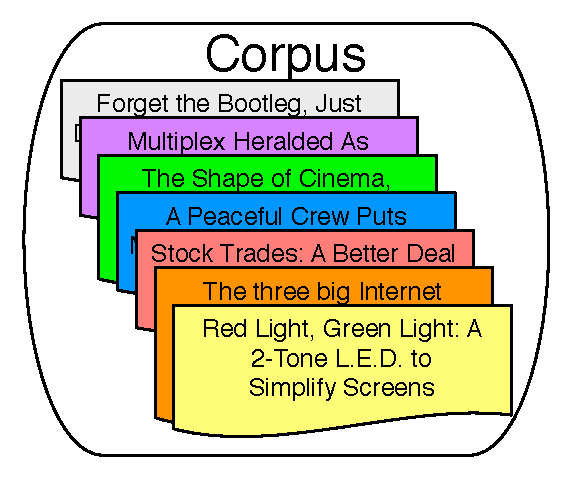
\includegraphics[width=0.6\linewidth]{reading_tea_leaves/figures/heldout_0} }
\only<2>{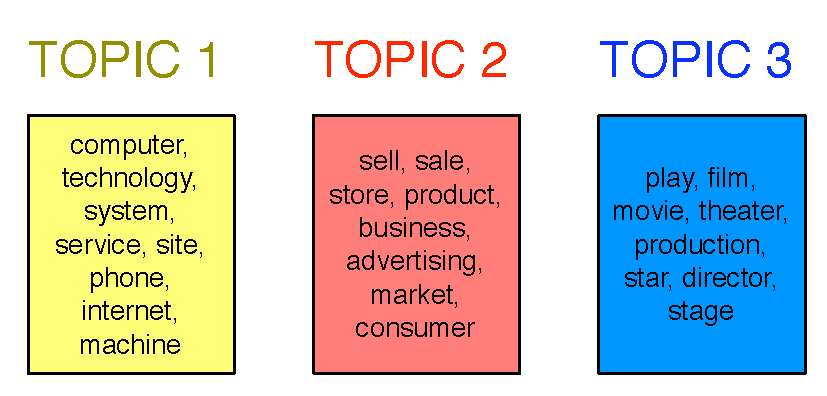
\includegraphics[width=0.9\linewidth]{reading_tea_leaves/figures/nyt_topics_wide}}
\only<3>{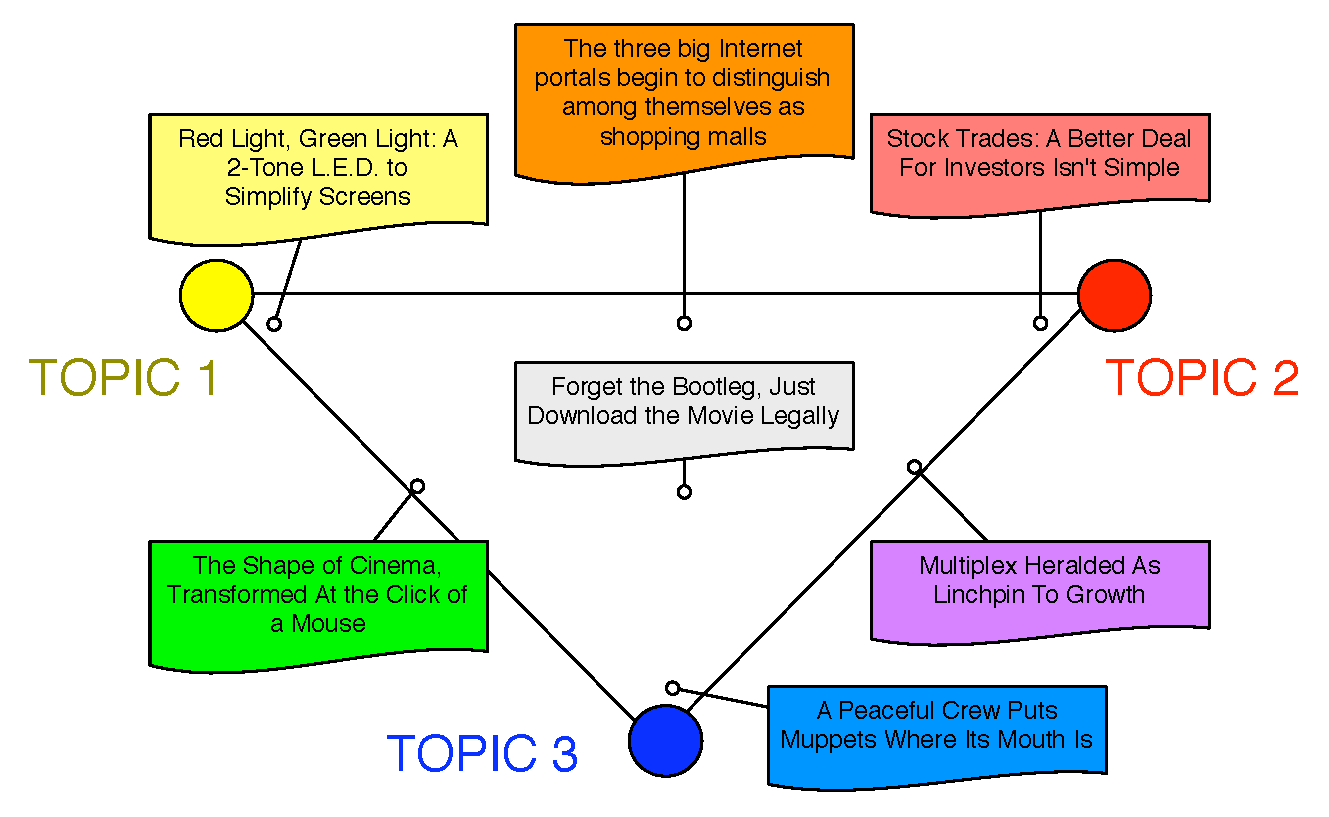
\includegraphics[width=0.9\linewidth]{topic_models/nyt_documents}}
\end{center}

\end{frame}


\begin{frame}
\frametitle{Topic Models in Academia}

\begin{columns}

\column{.6\linewidth}

\begin{itemize}
  \item Useful
    \begin{itemize}
      \item Computer Vision \cite{feifei-05}
      \item Social Networks \cite{airoldi-08}
      \item Music \cite{hu-09}
      \item Cognitive Science \cite{griffiths-06}
    \end{itemize}

\begin{block}{Latent Dirichlet Allocation}
Blei, Ng, and Jordan.  Journal of Machine Learning Research, 2003.
\end{block}


  \item Popular: most cited on Mendeley
  \item Easy: reasonable undergrad programming assignment
\end{itemize}


\column{.39\linewidth}
\begin{center}
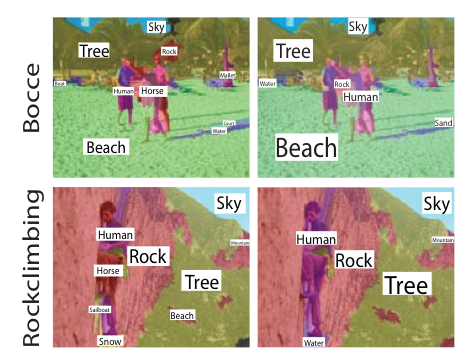
\includegraphics[width=0.8\linewidth]{topic_models/feifei} \\
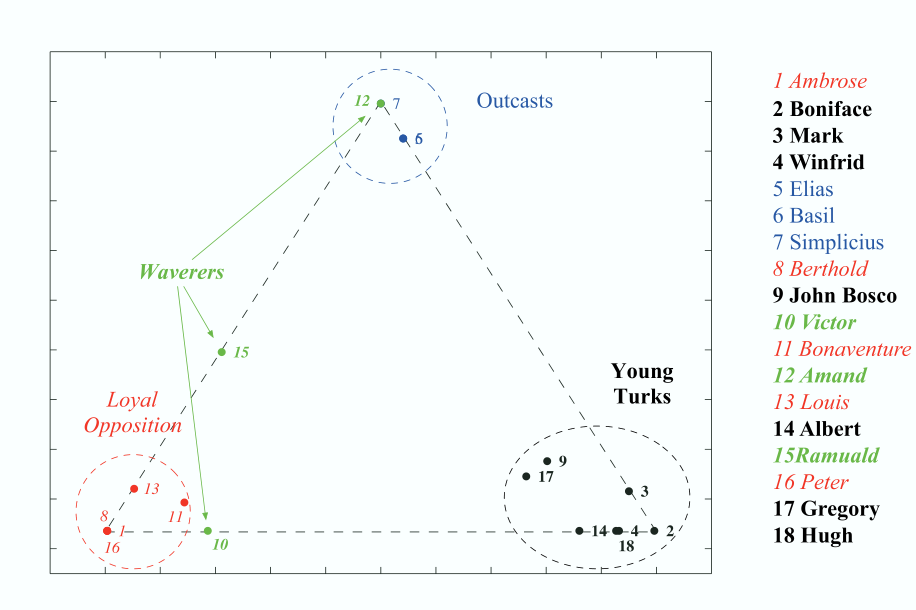
\includegraphics[width=0.8\linewidth]{topic_models/socialnetworks} \\
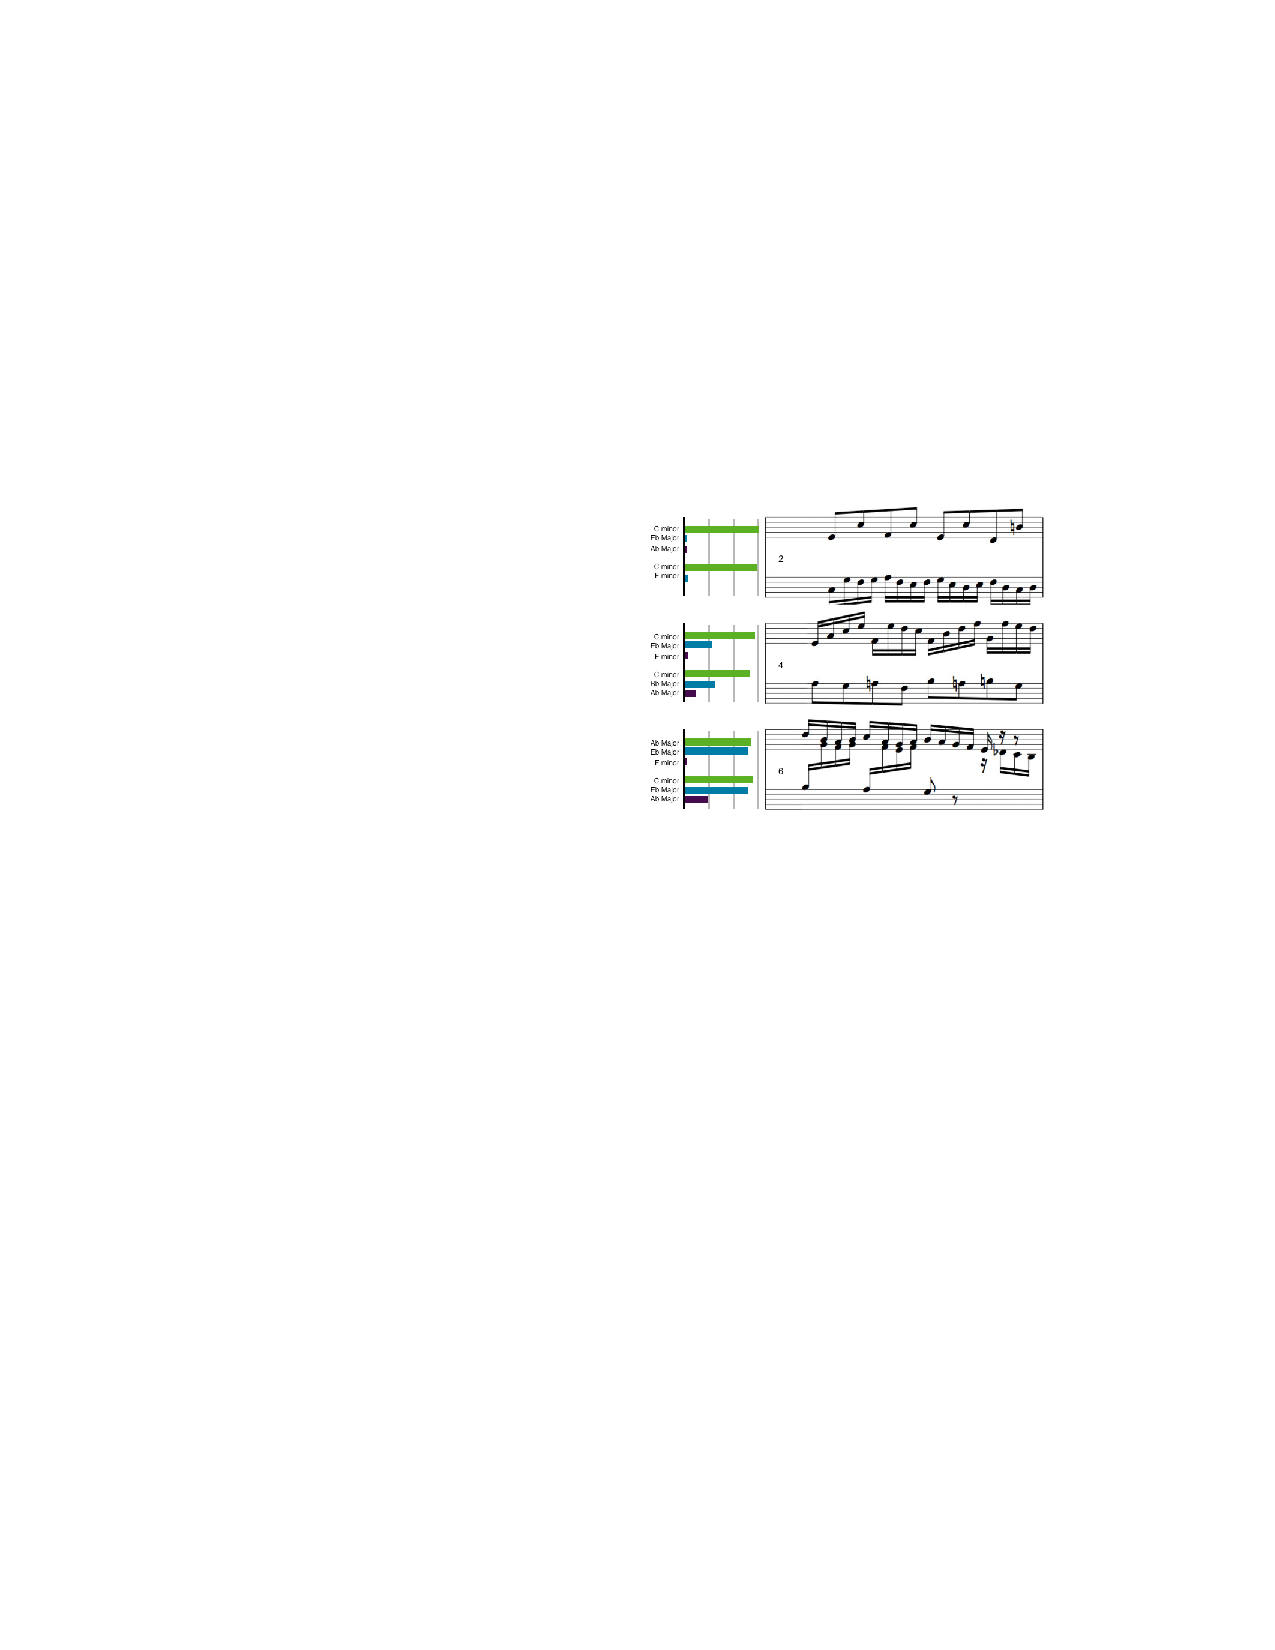
\includegraphics[width=0.8\linewidth]{topic_models/hu}
\end{center}
\end{columns}
\end{frame}

\begin{frame}
\frametitle{Topic Models in the Real World}

\vspace{-1cm}

\begin{columns}
  \column{.5\linewidth}
\begin{center}
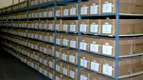
\includegraphics[width=0.8\linewidth]{topic_models/tobacco_litigation} \\
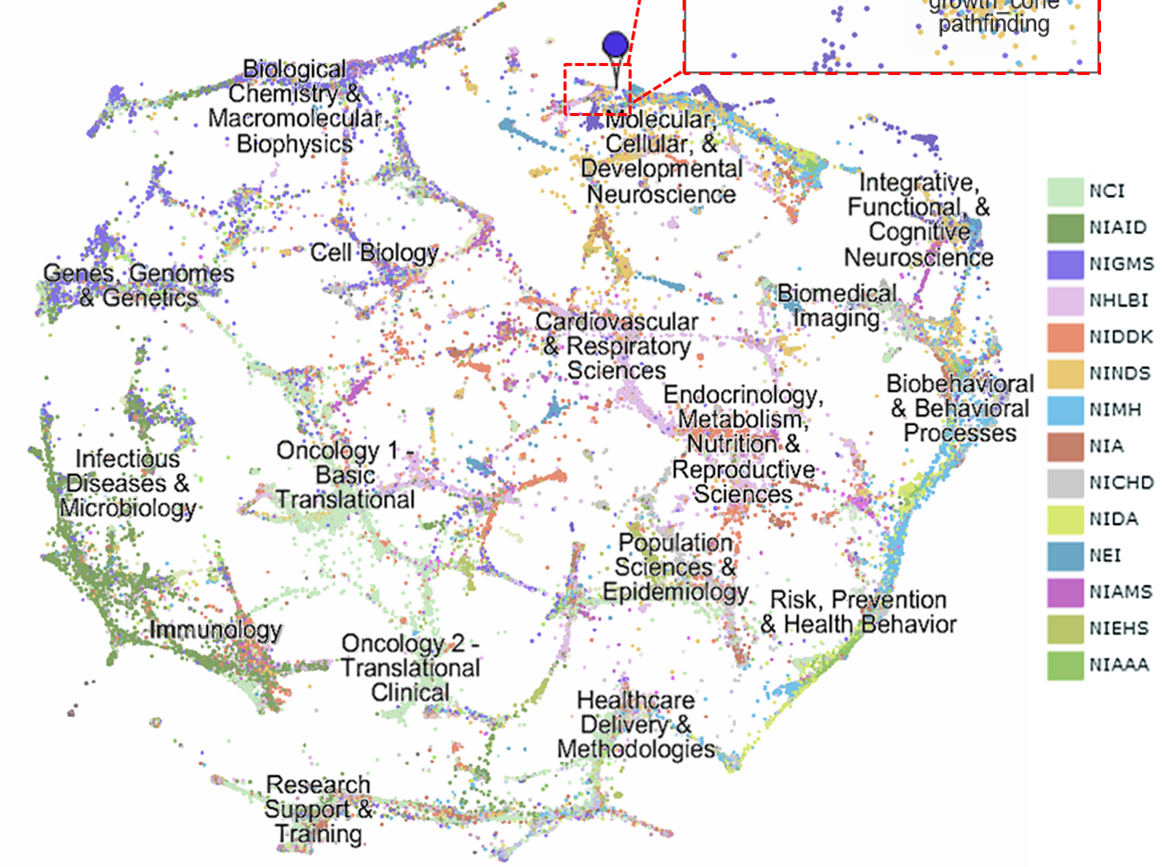
\includegraphics[width=0.8\linewidth]{topic_models/nih_topics} \\

\includegraphics[width=0.7\linewidth]{topic_models/sentiment}
\end{center}

  \column{.5\linewidth}

  \begin{itemize}
    \item E-discovery
    \item Understanding funding decisions
    \item Social media monitoring and sentiment analysis
  \end{itemize}

\end{columns}

\end{frame}

%

\providecommand{\graphscale}{0.6}


\newcommand{\dirfunc}[3]{ \frac{ \prod_{#1}^{#2} \g{ #3 } } { \g{ \sum_{#1}^{#2} #3 }}}
\newcommand{\dirnum}[4]{ \frac{\g{ #3 }}{#4} \prod_{#1}^{#2} }
\newcommand{\dirden}[3]{ \g{ \sum_{#1}^{#2} #3 } }

\section{Topic Model Introduction}

\begin{frame}

	\frametitle{Why topic models?}

	\begin{columns}

	\column{.3\linewidth}

	
\includegraphics[width=1\linewidth]{topic_models/newspapers}

	\column{.55\linewidth}

	\begin{itemize}
		\item Suppose you have a huge number of documents
		\item Want to know what's going on
		\item Can't read them all (e.g. every New York Times article from the 90's)
		\item Topic models offer a way to get a corpus-level view of major themes
		\pause
		\item Unsupervised
	\end{itemize}


	\end{columns}

\end{frame}

\frame{
\begin{center}
\frametitle{Conceptual Approach}
From an \textbf<1>{input corpus} and number of topics \textbf<1>{$K$} $\rightarrow$ \textbf<2>{words to topics} \\
\only<1>{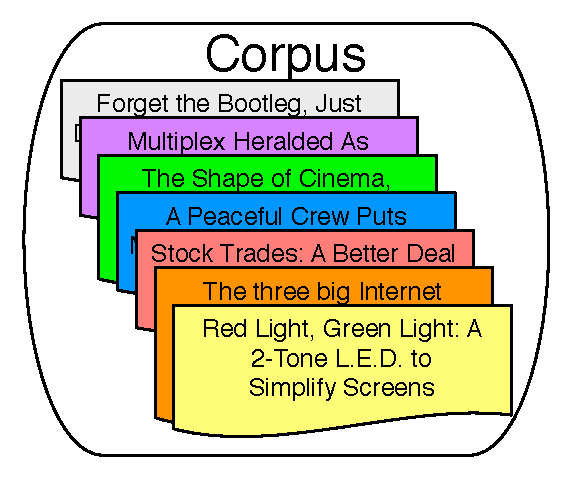
\includegraphics[width=0.6\linewidth]{reading_tea_leaves/figures/heldout_0} }
\only<2>{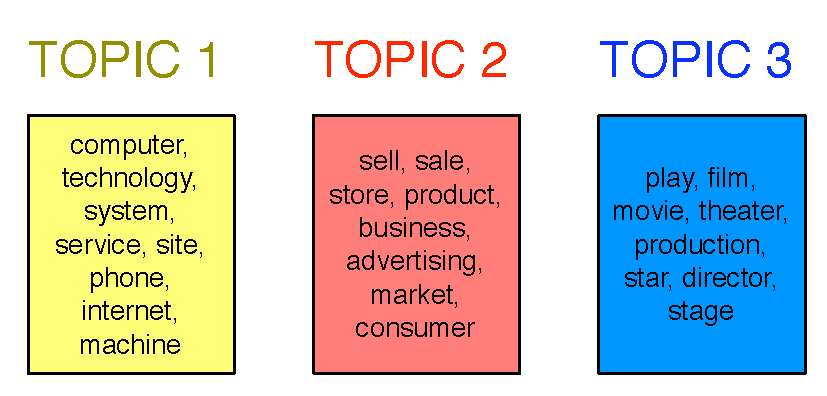
\includegraphics[width=0.9\linewidth]{reading_tea_leaves/figures/nyt_topics_wide}}
\end{center}
}

\frame{\frametitle{Conceptual Approach}

\begin{itemize}
\item For each document, what topics are expressed by that document?

\begin{center}
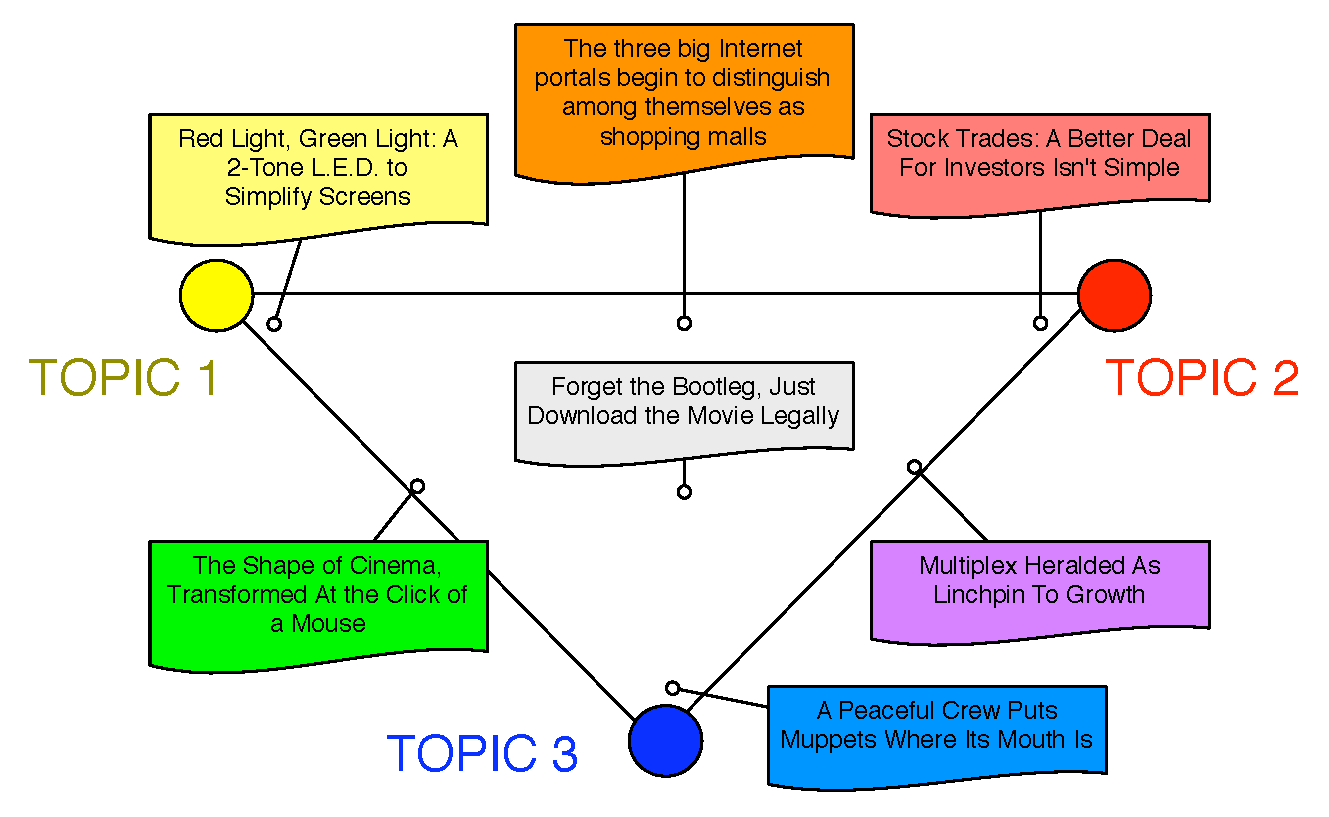
\includegraphics[width=0.9\linewidth]{topic_models/nyt_documents}
\end{center}

\end{itemize}
}

\iflong

\begin{frame}

\frametitle{Topics from \emph{Science}}

\begin{center}
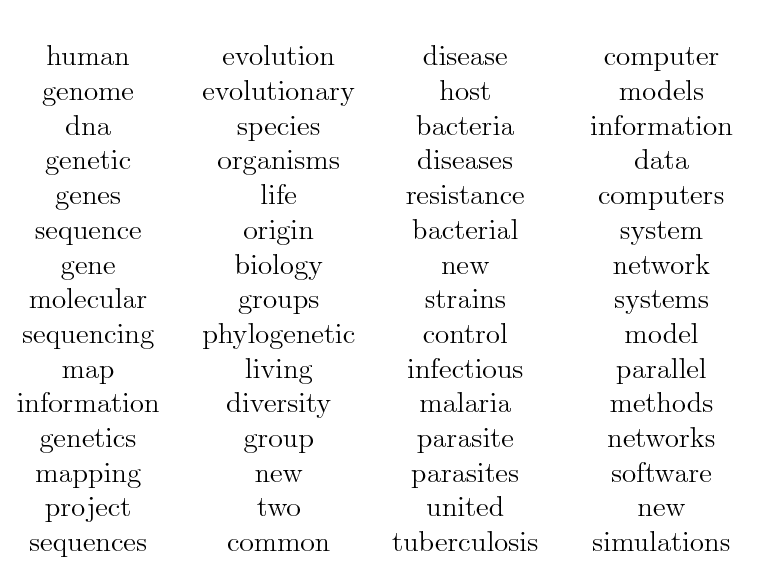
\includegraphics[width=0.8\linewidth]{topic_models/example_topics}
\end{center}

\end{frame}


\begin{frame}

\frametitle{Why should you care?}

\begin{itemize}
\item Neat way to explore / understand corpus collections
\begin{itemize}
	\item E-discovery
	\item Social media
	\item Scientific data
\end{itemize}
\item NLP Applications
\begin{itemize}
   \item POS Tagging~\cite{toutanova-08}
   \item Word Sense Disambiguation~\cite{boyd-graber-07}
   \item Word Sense Induction~\cite{brody-09}
   \item Discourse Segmentation~\cite{purver-06}
\end{itemize}
\item Psychology~\cite{griffiths-07}: word meaning, polysemy
\item Inference is (relatively) simple
\end{itemize}

\end{frame}

\frame
{
  \frametitle{Matrix Factorization Approach}

\begin{center}
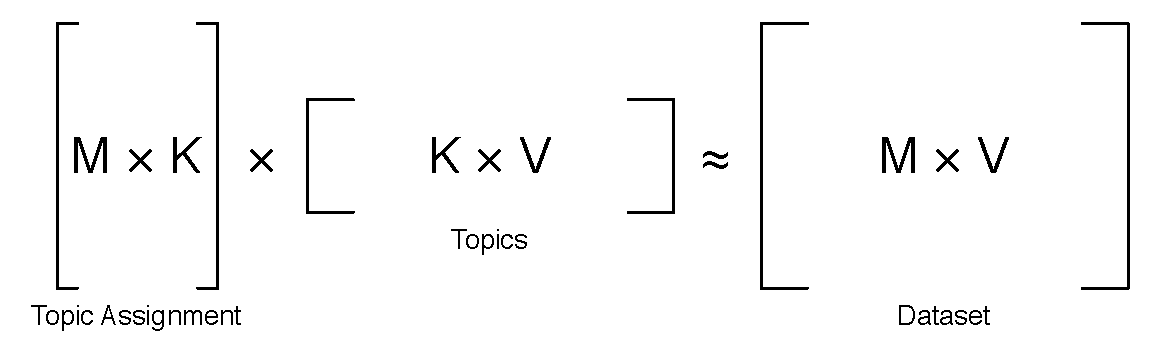
\includegraphics[width=0.9\linewidth]{topic_models/factorization.pdf}
\end{center}

\begin{columns}
\column{.5\textwidth}
\begin{block}{}
	\begin{itemize}
		\item[K] Number of topics
		\item[M] Number of documents
		\item[V] Size of vocabulary
	\end{itemize}
\end{block}
\column{.5\textwidth}
\pause
\begin{itemize}
\item If you use singular value decomposition (SVD), this technique is called latent semantic analysis.
\item Popular in information retrieval.
\end{itemize}
\end{columns}

}

\begin{frame}

\frametitle{Alternative: Generative Model}

\begin{itemize}
  \item How your data came to be
  \item Sequence of Probabilistic Steps
  \item Posterior Inference
\end{itemize}

\end{frame}

\begin{frame}
	\frametitle{Multinomial Distribution}

	\begin{itemize}
		\item Distribution over discrete outcomes
		\item Represented by non-negative vector that sums to one
		\item Picture representation
	\begin{center}
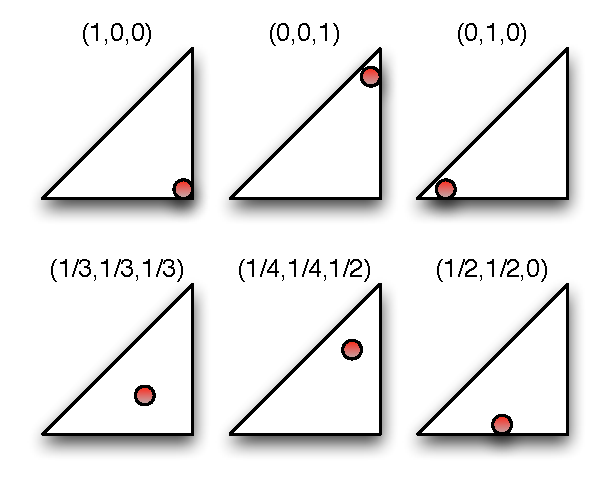
\includegraphics[width=0.4\linewidth]{topic_models/multinomial}
	\end{center}
		\pause
		\item Come from a Dirichlet distribution

	\end{itemize}


\end{frame}

\begin{frame}

\frametitle{Dirichlet Distribution}

\begin{center}
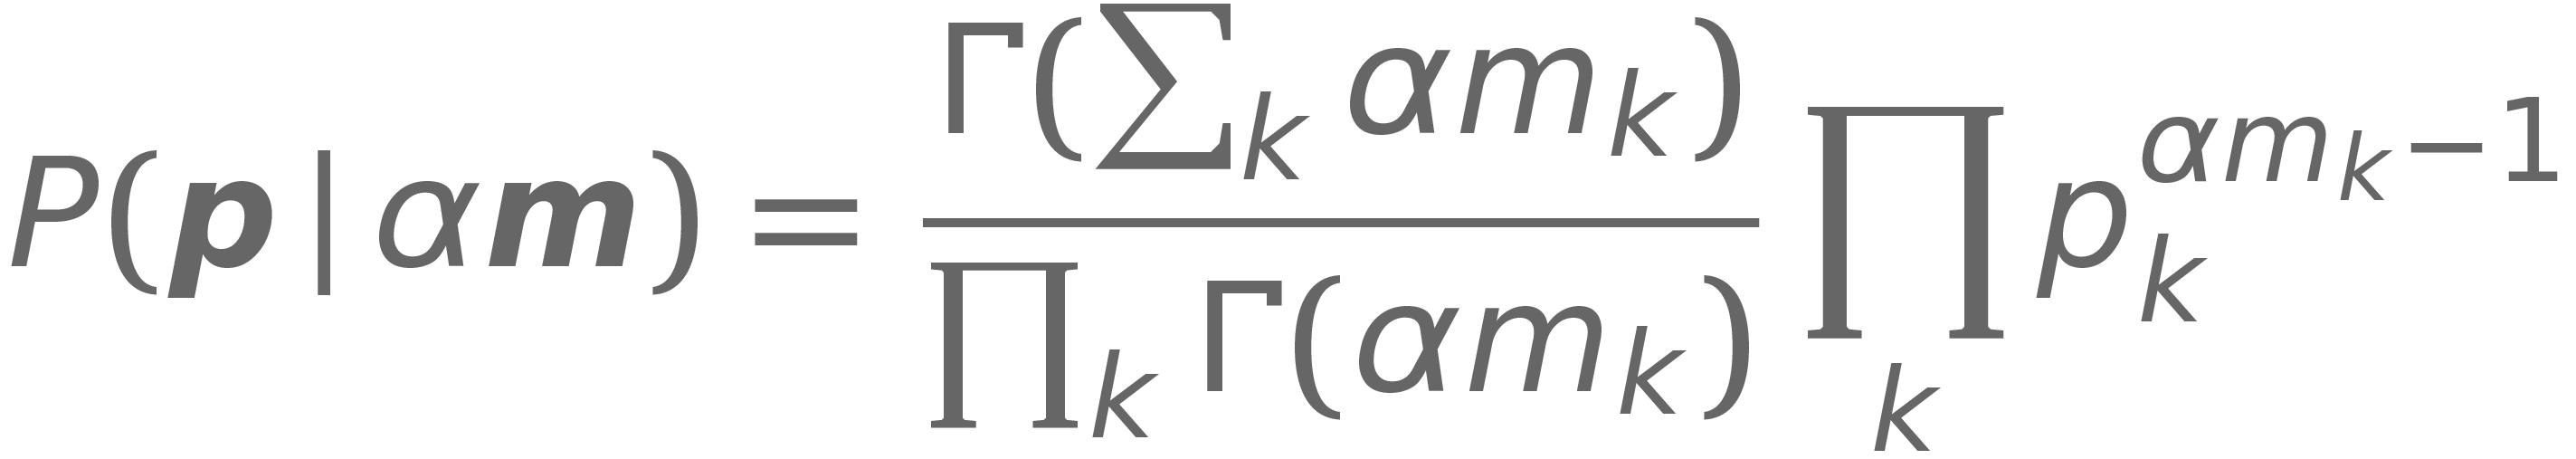
\includegraphics[width=0.4\linewidth]{topic_models/equations/dirichlet} \\ \bigskip
\pause

\includegraphics[width=0.6\linewidth]{topic_models/dirichlet_1} \\
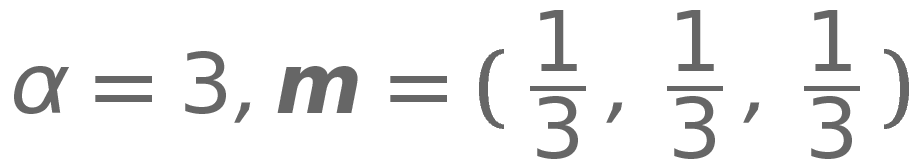
\includegraphics[width=0.2\linewidth]{topic_models/equations/dirichlet_params_1} 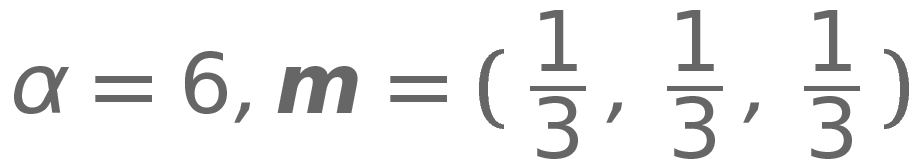
\includegraphics[width=0.2\linewidth]{topic_models/equations/dirichlet_params_2} 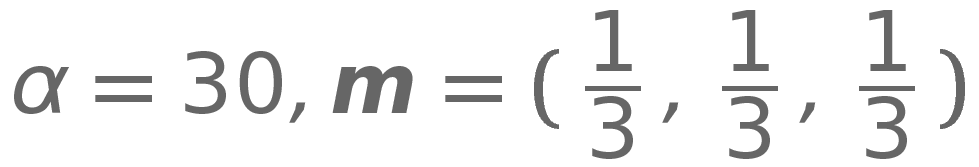
\includegraphics[width=0.2\linewidth]{topic_models/equations/dirichlet_params_3} \\
\pause

\includegraphics[width=0.6\linewidth]{topic_models/dirichlet_2} \\
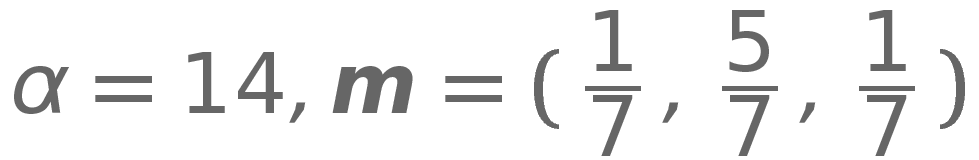
\includegraphics[width=0.2\linewidth]{topic_models/equations/dirichlet_params_4} 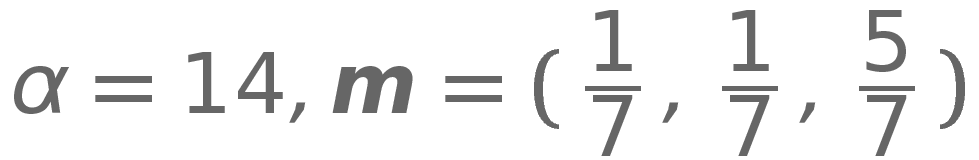
\includegraphics[width=0.2\linewidth]{topic_models/equations/dirichlet_params_5} 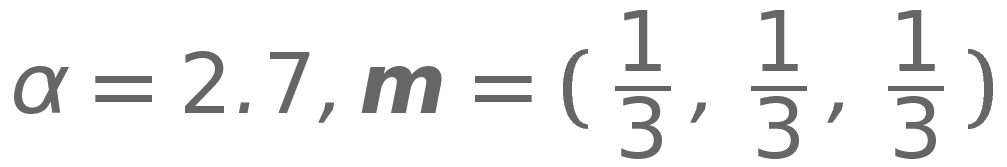
\includegraphics[width=0.2\linewidth]{topic_models/equations/dirichlet_params_6} \\
\end{center}

\end{frame}

\begin{frame}
\frametitle{Dirichlet Distribution}
\begin{center}
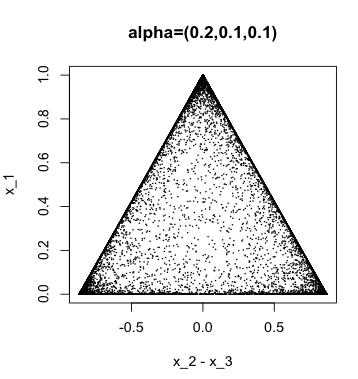
\includegraphics[width=0.5\linewidth]{topic_models/sparsity}
\end{center}
\end{frame}

\fi
\ifconjugacy

\begin{frame}
\frametitle{Dirichlet Distribution}
\begin{itemize}
  \item If ${\bm \phi} \sim \Dir(\alpha)$, ${\bm w} \sim \Mult(\phi)$, and $n_k = |\{ w_i : w_i = k\}|$ then
  \begin{align}
  	p(\phi | \alpha, {\bm w}) & \propto p({\bm w} | \phi) p(\phi | \alpha) \\
	                       & \propto  \prod_{k} \phi^{n_k} \pause  \prod_k { \phi^{\alpha_k - 1}} \\
	                       & \propto \prod_k \phi^{\alpha_k + n_k - 1}
  \end{align}
  \item Conjugacy: this {\bf posterior} has the same form as the {\bf prior}
\end{itemize}
\end{frame}

\fi

\ifhighlevel

\else

\frame
{
  \frametitle{Generative Model Approach}

\begin{center}
\only<1>{ 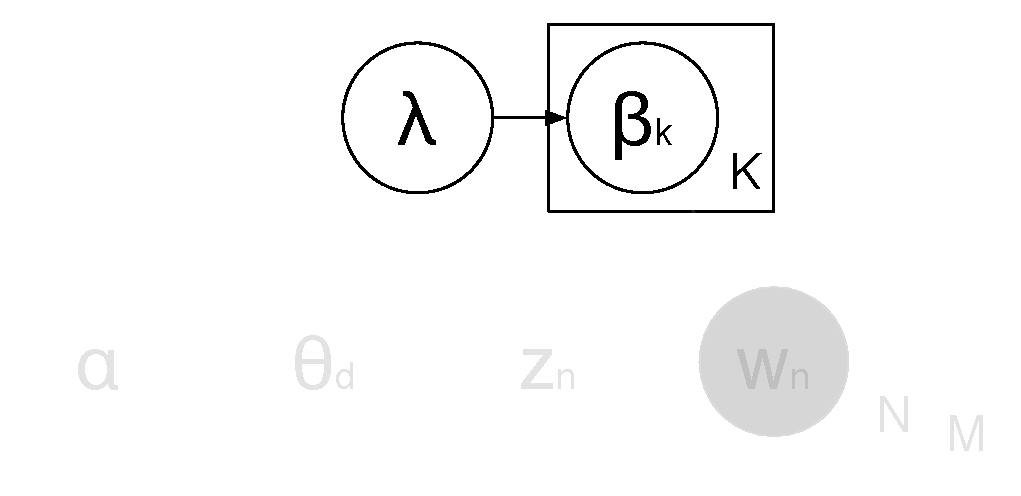
\includegraphics[scale=0.4]{topic_models/lda1.pdf} }
\only<2>{ 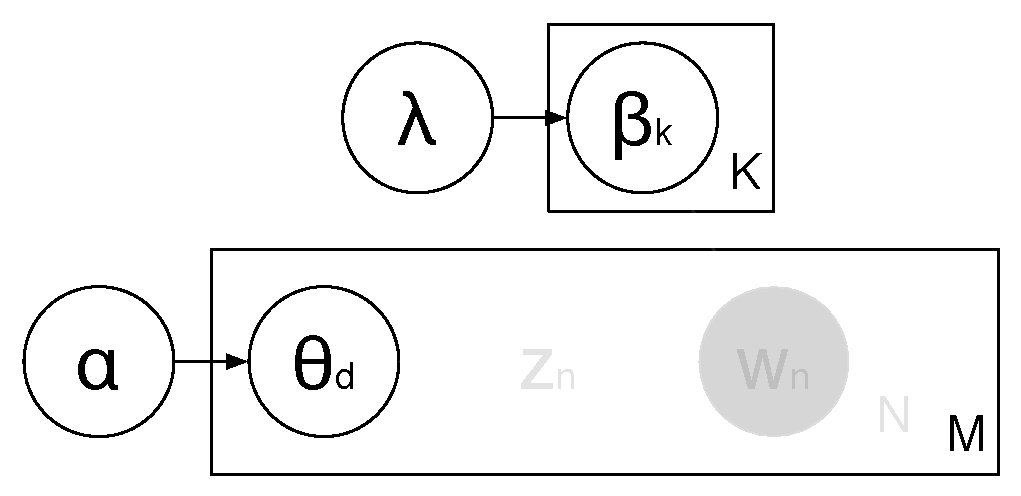
\includegraphics[scale=0.4]{topic_models/lda2.pdf} }
\only<3>{ 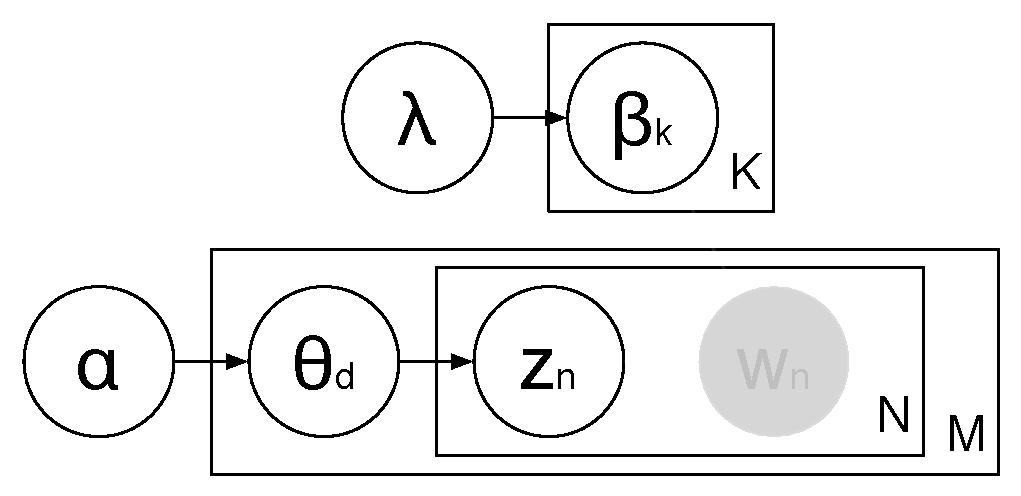
\includegraphics[scale=0.4]{topic_models/lda3.pdf} }
\only<4->{ 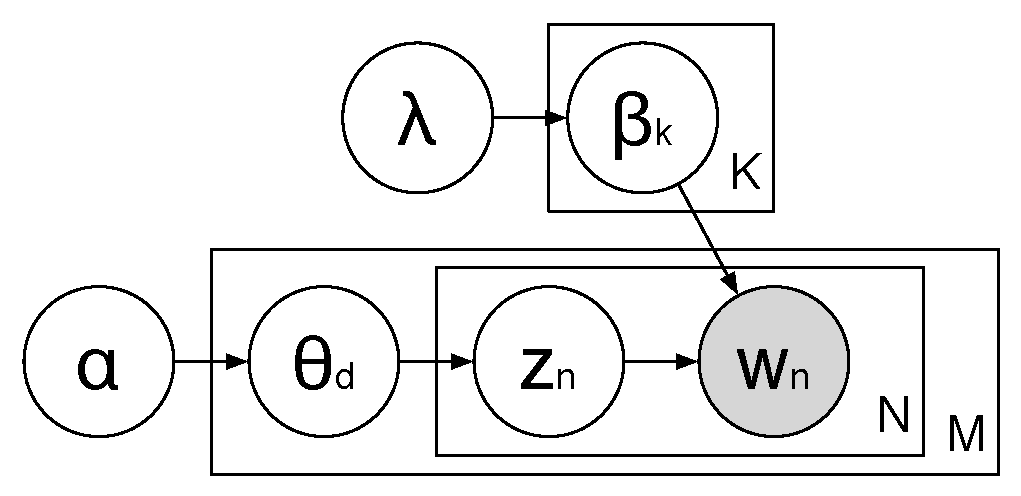
\includegraphics[scale=0.4]{topic_models/lda4.pdf} }
\end{center}

\begin{itemize}
\item<1-> For each topic $k \in \{1, \dots, K\}$, draw a multinomial distribution $\beta_k$ from a Dirichlet distribution with parameter $\lambda$
\item<2-> For each document $d \in \{1, \dots, M\}$, draw a multinomial distribution $\theta_d$ from a Dirichlet distribution with parameter $\alpha$
\item<3-> For each word position $n \in \{1, \dots, N\}$, select a hidden topic $z_n$ from the multinomial distribution parameterized by $\theta$.
\item<4-> Choose the observed word $w_n$ from the distribution $\beta_{z_n}$.
\end{itemize}

\only<5->{We use statistical inference to uncover the most likely unobserved variables given observed data.}
}

\fi

\begin{frame}
\frametitle{Topic Models: What's Important}
\begin{itemize}
\item Topic models \only<2>{(latent variables)}
\begin{itemize}
\ifhighlevel
	\item Topics to words
	\item Documents to topics
\else
	\item Topics to words---multinomial distribution
	\item Documents to topics---multinomial distribution
\fi
\end{itemize}
\item Focus in this talk: statistical methods
  \begin{itemize}
    \item Model: story of how your data came to be
    \item Latent variables: missing pieces of your story
    \item Statistical inference: filling in those missing pieces
  \end{itemize}
\item We use latent Dirichlet allocation (LDA)~\cite{blei-03}, a fully Bayesian
  version of pLSI~\cite{hofmann-99}, probabilistic version of
  LSA~\cite{landauer-97}
\end{itemize}

\end{frame}

\ifevaluation


\frame{
\frametitle{Evaluation}
\begin{center}
%\only<1>{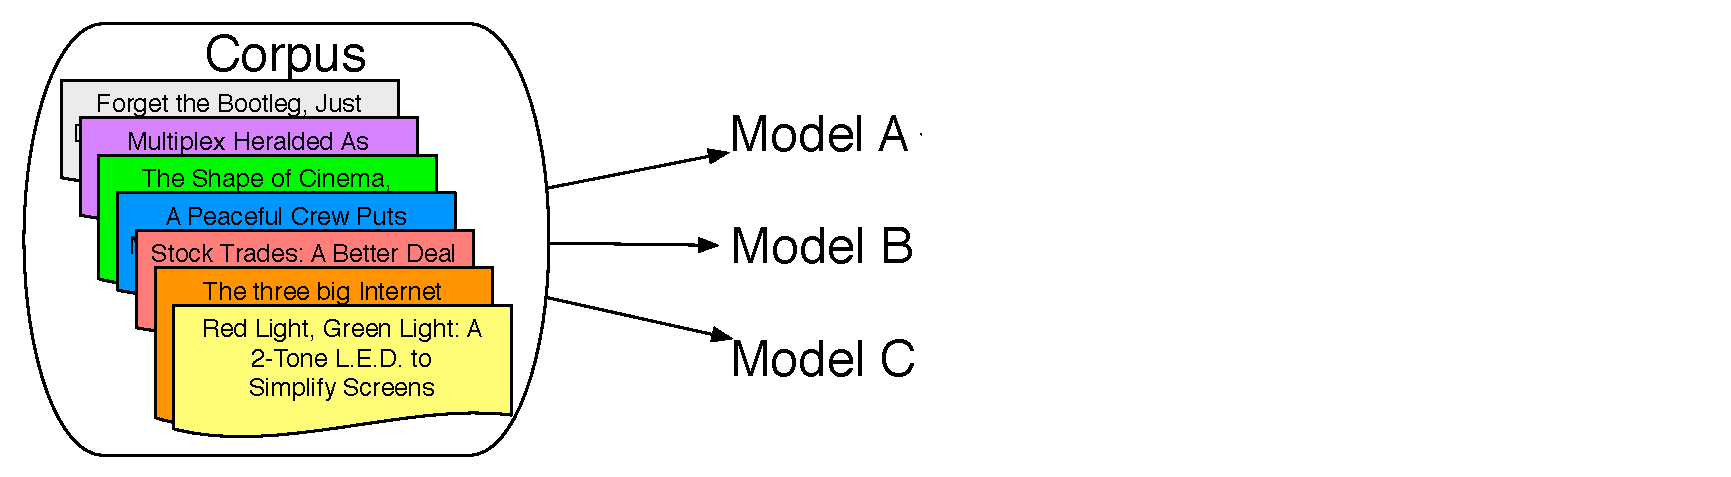
\includegraphics[width=0.9\linewidth]{reading_tea_leaves/figures/heldout_1} }
\only<1>{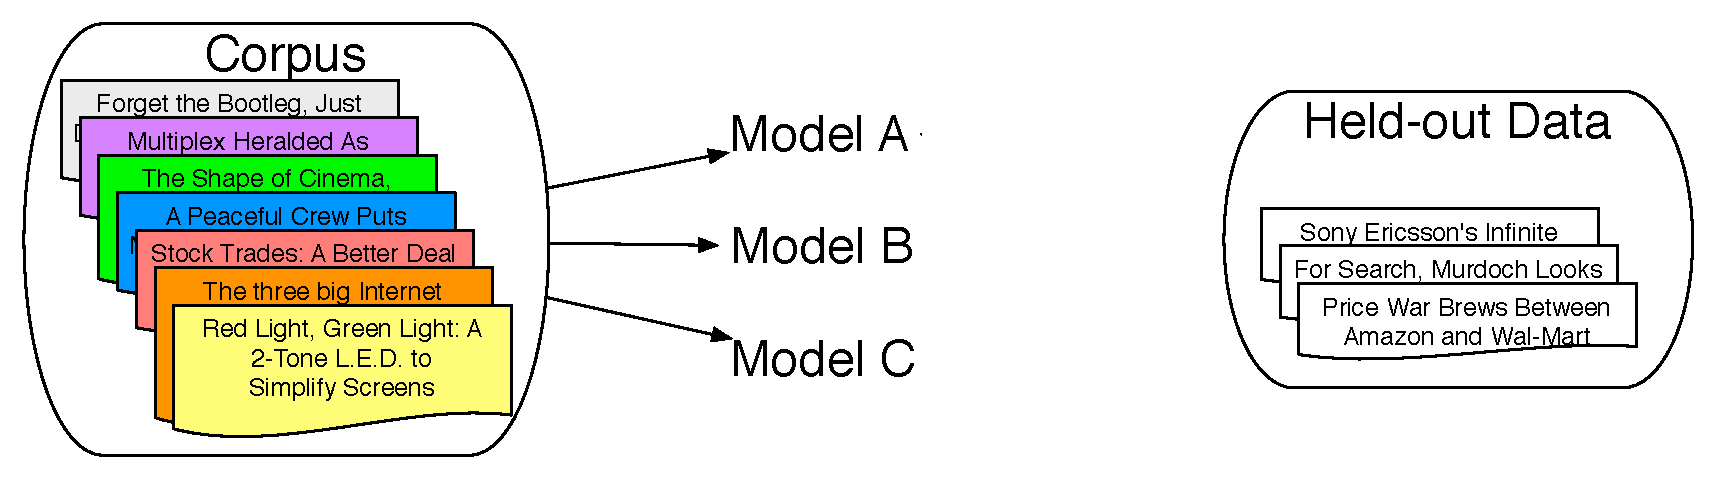
\includegraphics[width=\linewidth]{reading_tea_leaves/figures/heldout_2} }
%\only<3>{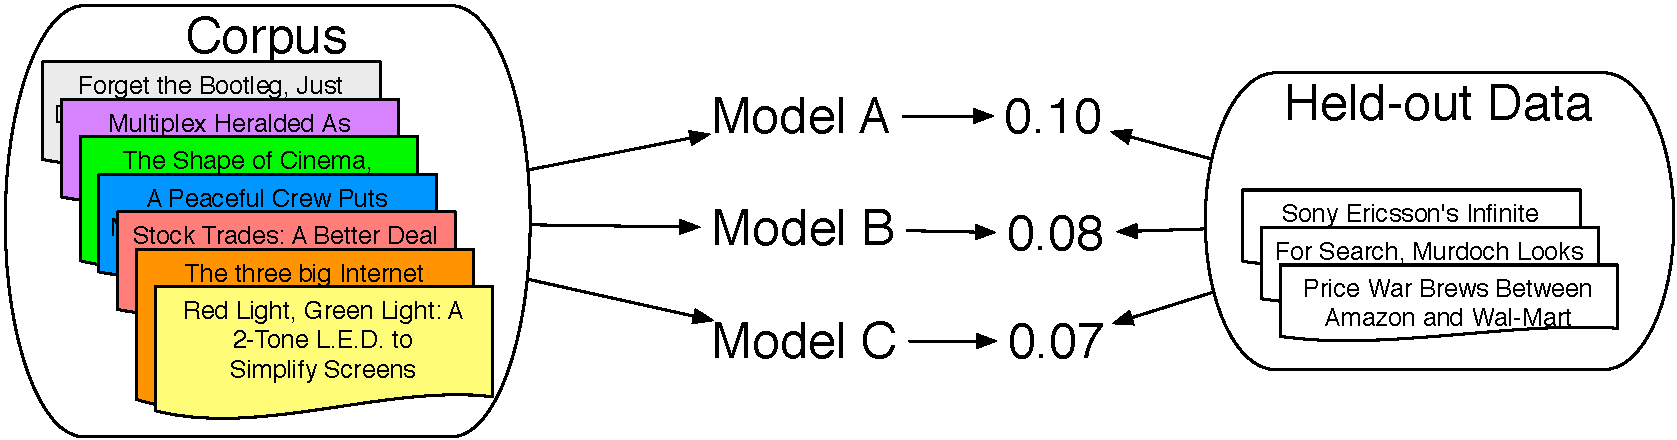
\includegraphics[width=\linewidth]{reading_tea_leaves/figures/heldout_3} }
\only<2>{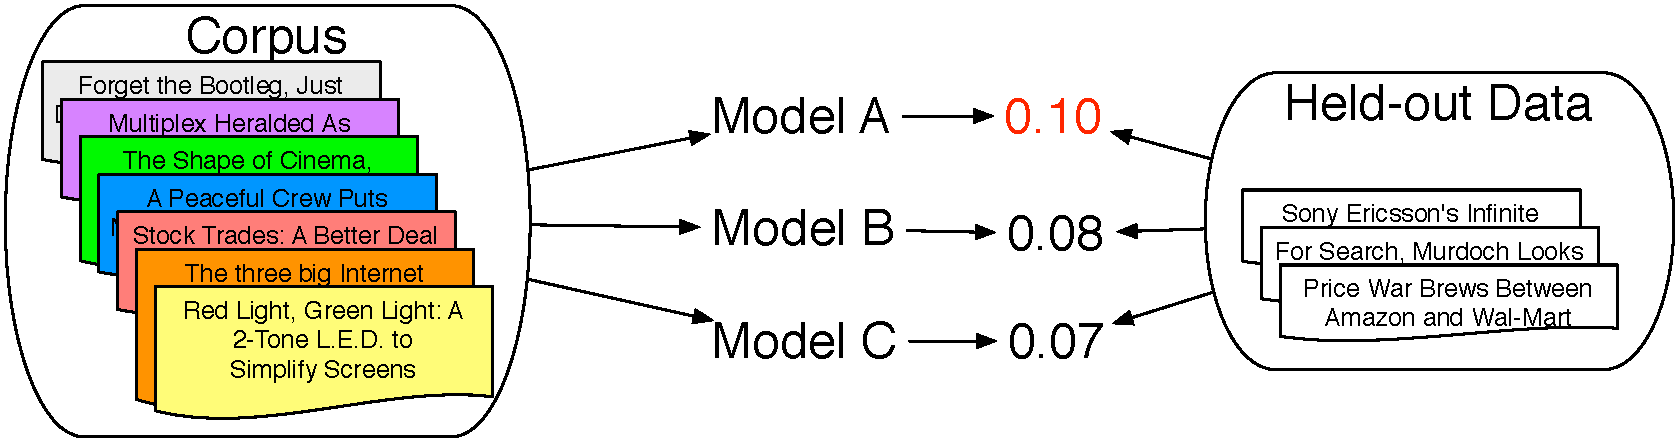
\includegraphics[width=\linewidth]{reading_tea_leaves/figures/heldout_4}  \\
	\large Measures predictive power, not what the topics are}
\end{center}

\begin{center}
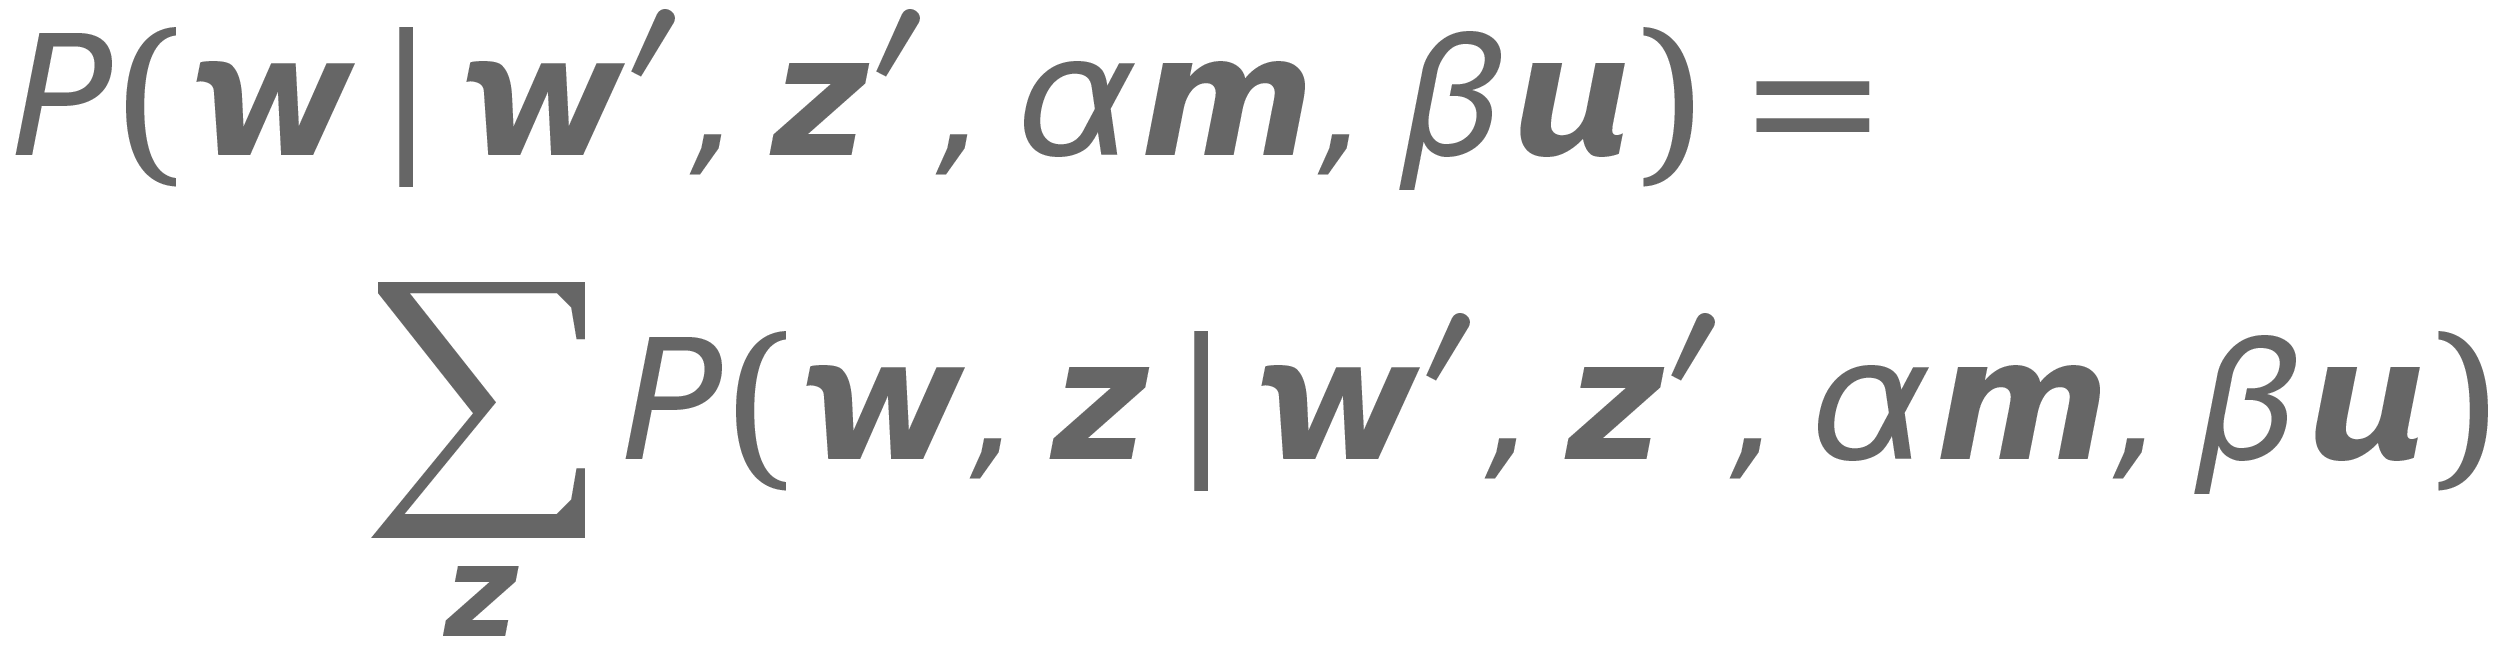
\includegraphics[width=0.5\linewidth]{topic_models/equations/evaluation} \\
How you compute it is important too~\cite{wallach-09b}
\end{center}

}

\frame{
  \frametitle{Word Intrusion}

  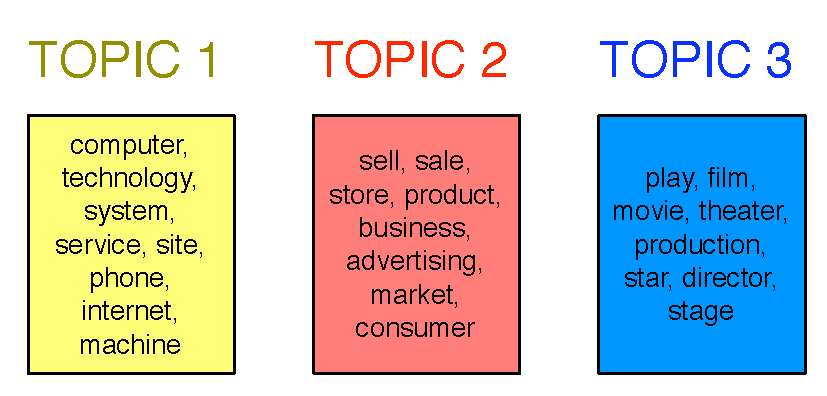
\includegraphics[width=\linewidth]{reading_tea_leaves/figures/nyt_topics_wide}
}


\frame{
  \frametitle{Word Intrusion}

  \begin{enumerate}
    \item Take the highest probability words from a topic

      \begin{block}{Original Topic}
        dog, cat, horse, pig, cow
      \end{block}
\pause
    \item Take a high-probability word from another topic and add it
      \begin{block}{Topic with Intruder}
        dog, cat, \alert<2->{apple}, horse, pig, cow
      \end{block}
\pause
     \item We ask users to find the word that doesn't belong
  \end{enumerate}
\begin{block}{Hypothesis}
If the topics are interpretable, users will consistently choose true intruder
\end{block}
}

\frame{
\frametitle{Word Intrusion}
\begin{center}
\only<1>{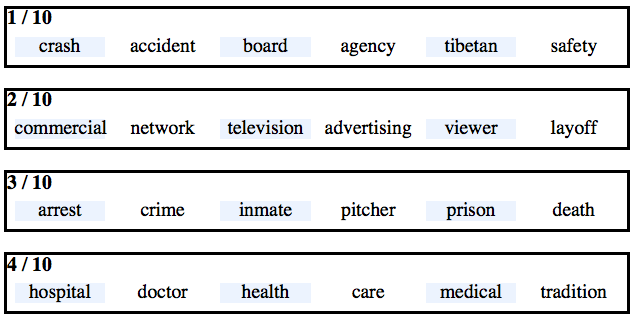
\includegraphics[width=\linewidth]{reading_tea_leaves/tasks/word1}  }
\only<2>{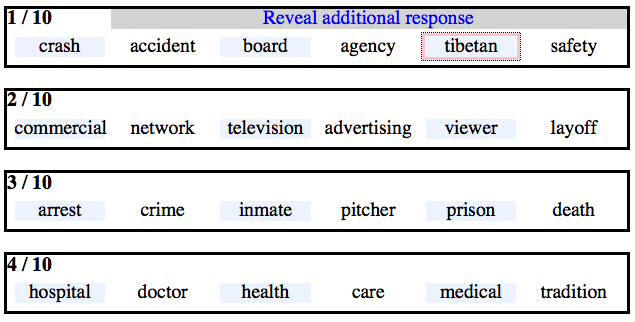
\includegraphics[width=\linewidth]{reading_tea_leaves/tasks/word2}  }
\pause
  \begin{itemize}
    \item Order of words was shuffled
    \item Which intruder was selected varied
    \item Model precision: percentage of users who clicked on intruder
  \end{itemize}

\end{center}
}

\frame{
\frametitle{Word Intrusion: Which Topics are Interpretable?}
  \begin{block}{New York Times, 50 LDA Topics}
    \begin{center}
      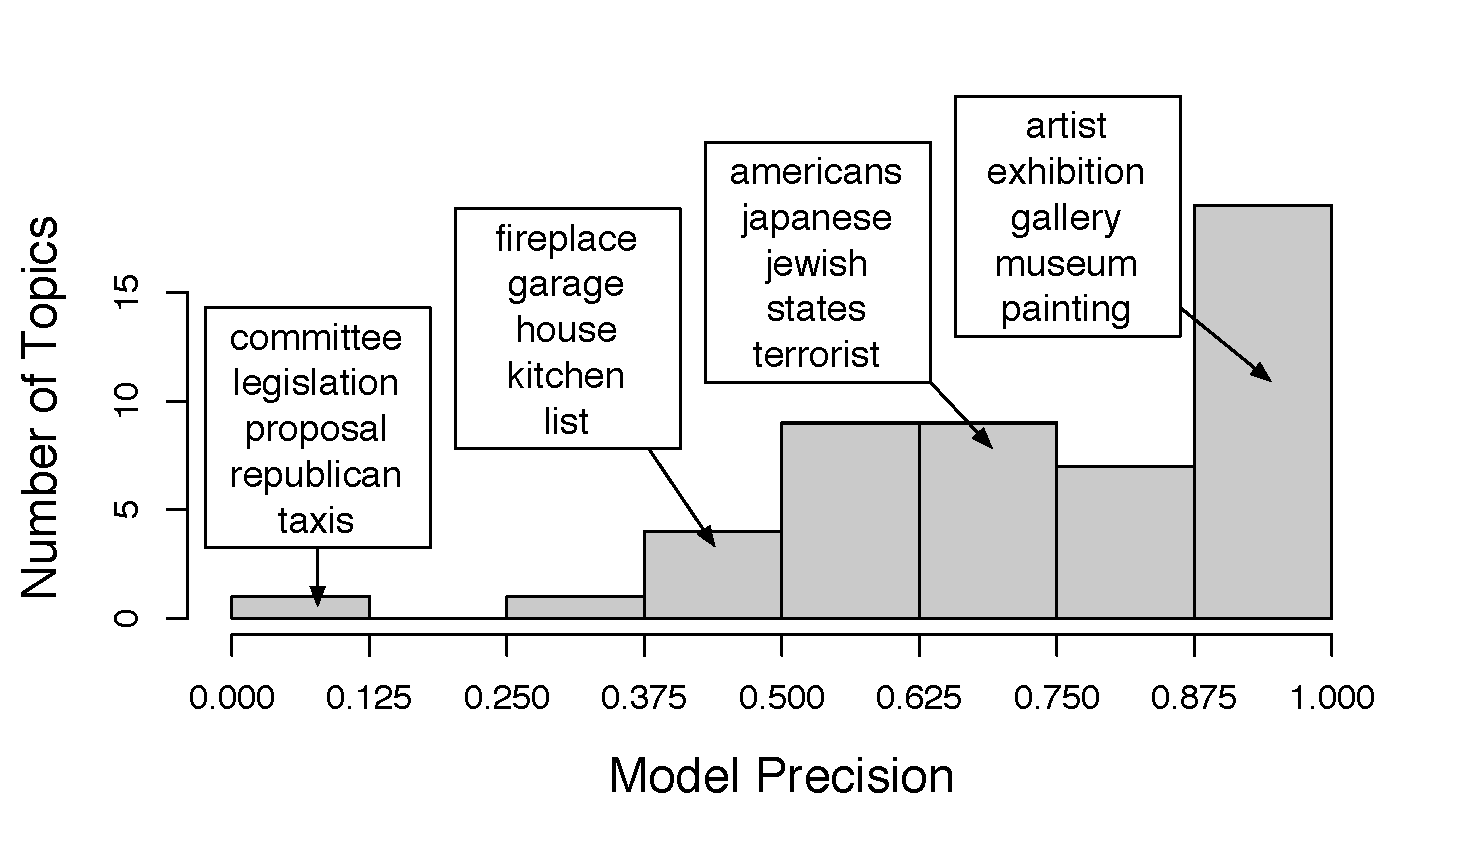
\includegraphics[width=0.8\linewidth]{reading_tea_leaves/figures/topic_precision}
    \end{center}
  \end{block}
  \begin{center}
    Model Precision: percentage of correct intruders found
  \end{center}
}



\frame{

\frametitle{Interpretability and Likelihood}
\begin{center}
\only<1>{Model Precision on New York Times}
\only<2>{Topic Log Odds on Wikipedia}
\end{center}

\begin{columns}
\column{.85\linewidth}
\begin{flushright}
  \only<1>{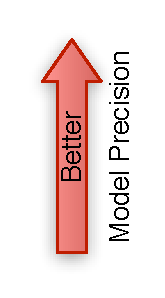
\includegraphics[scale=\graphscale]{reading_tea_leaves/tasks/mp}}
  \only<2>{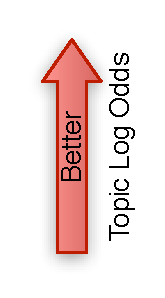
\includegraphics[scale=\graphscale]{reading_tea_leaves/tasks/tlo}}
  \only<1>{
\includegraphics[scale=\graphscale]{reading_tea_leaves/tasks/mp_y}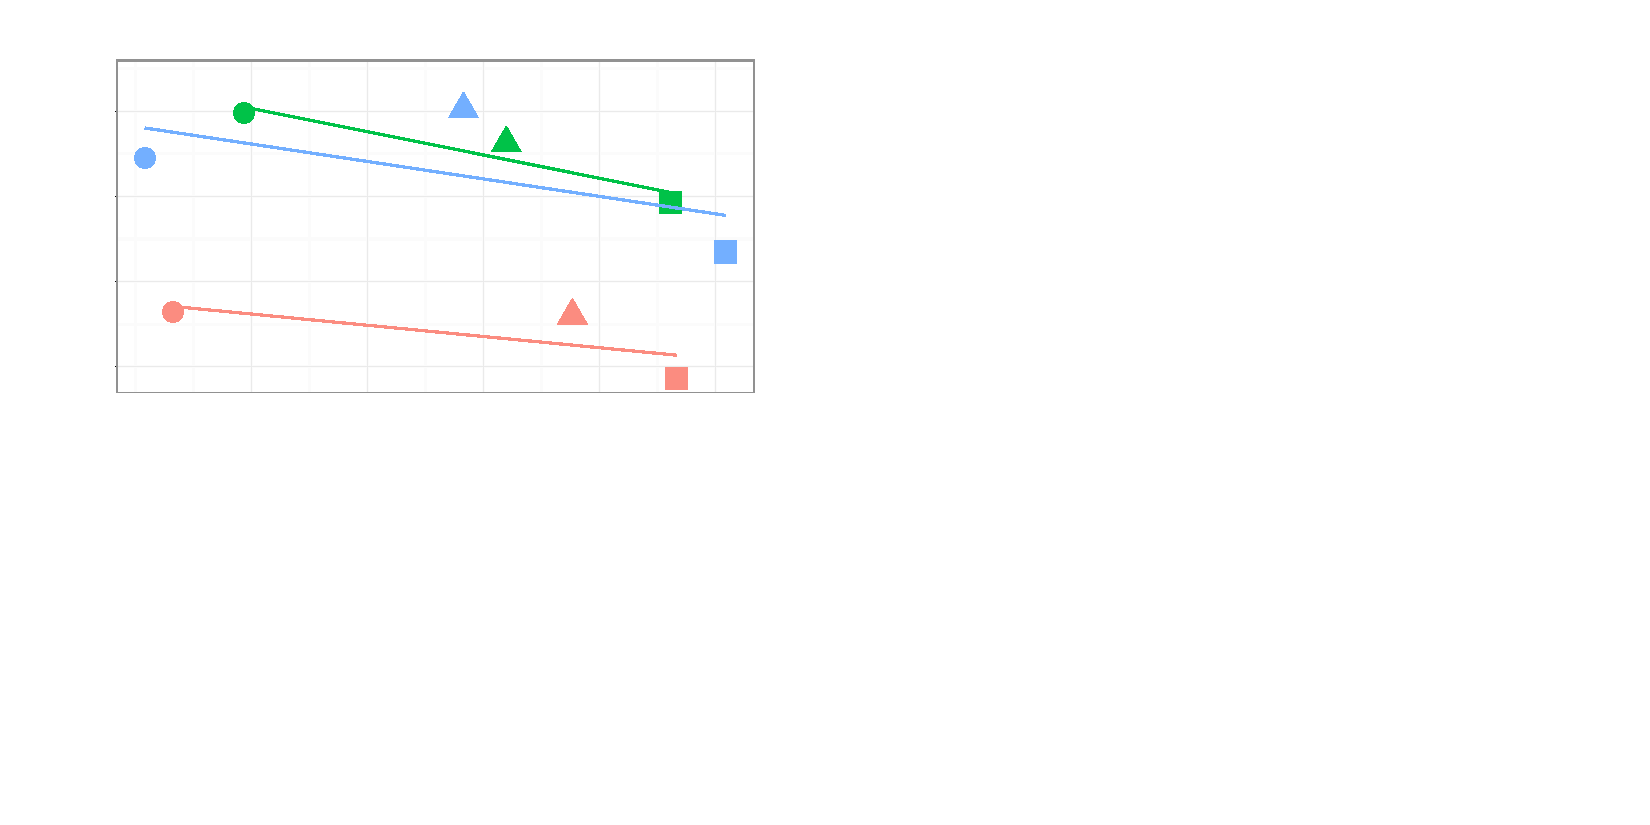
\includegraphics[scale=\graphscale]{reading_tea_leaves/tasks/nyt_mp}}
  \only<2>{
\includegraphics[scale=\graphscale]{reading_tea_leaves/tasks/tlo_y}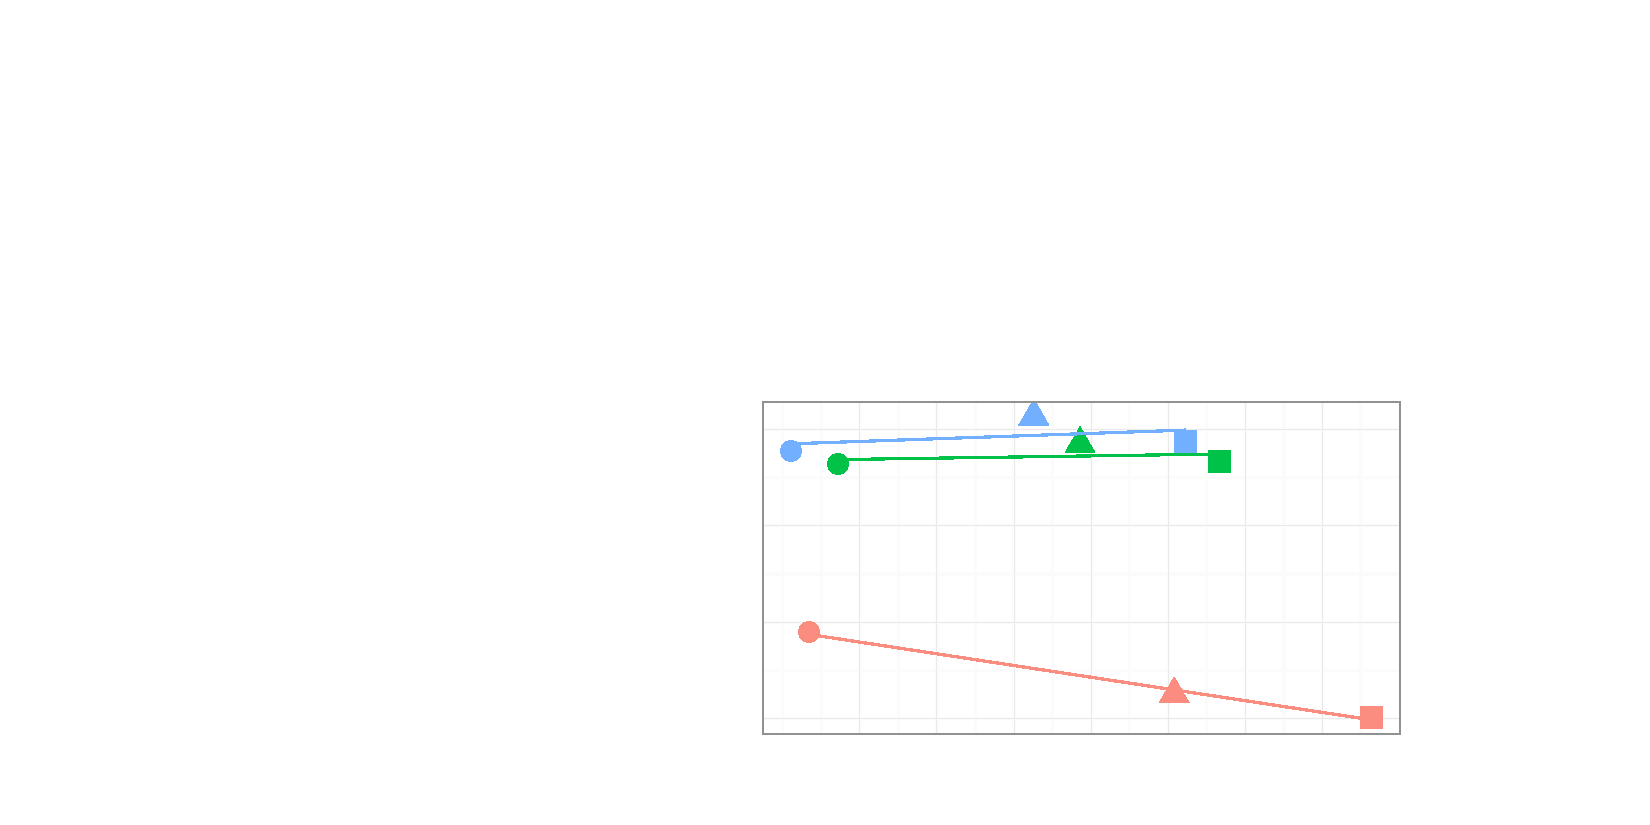
\includegraphics[scale=\graphscale]{reading_tea_leaves/tasks/wiki_tlo}} \\
  \only<1>{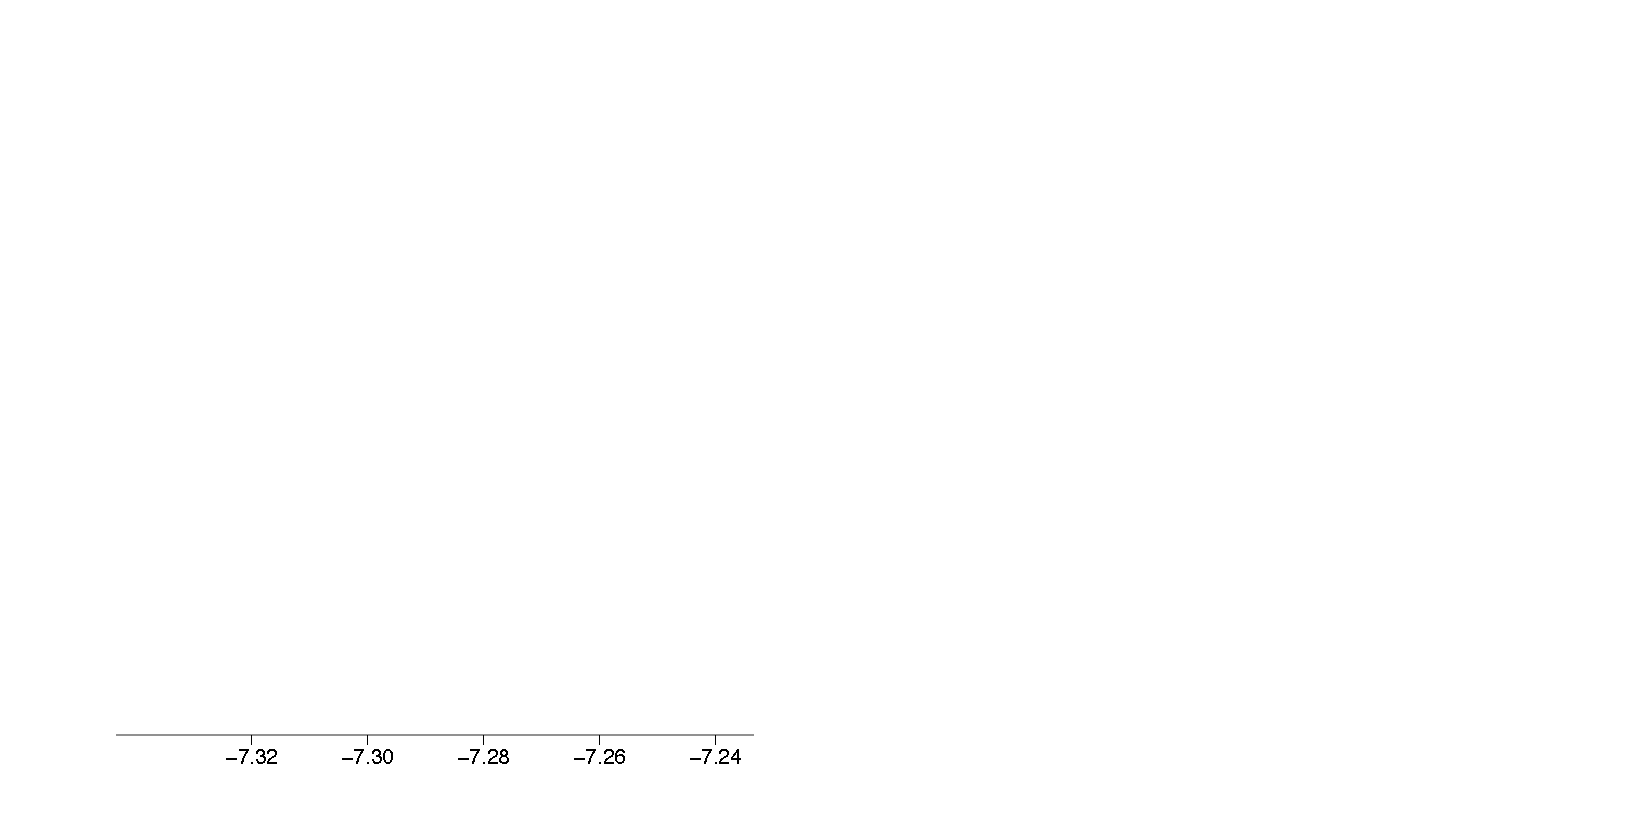
\includegraphics[scale=\graphscale]{reading_tea_leaves/tasks/nyt_x}}
  \only<2>{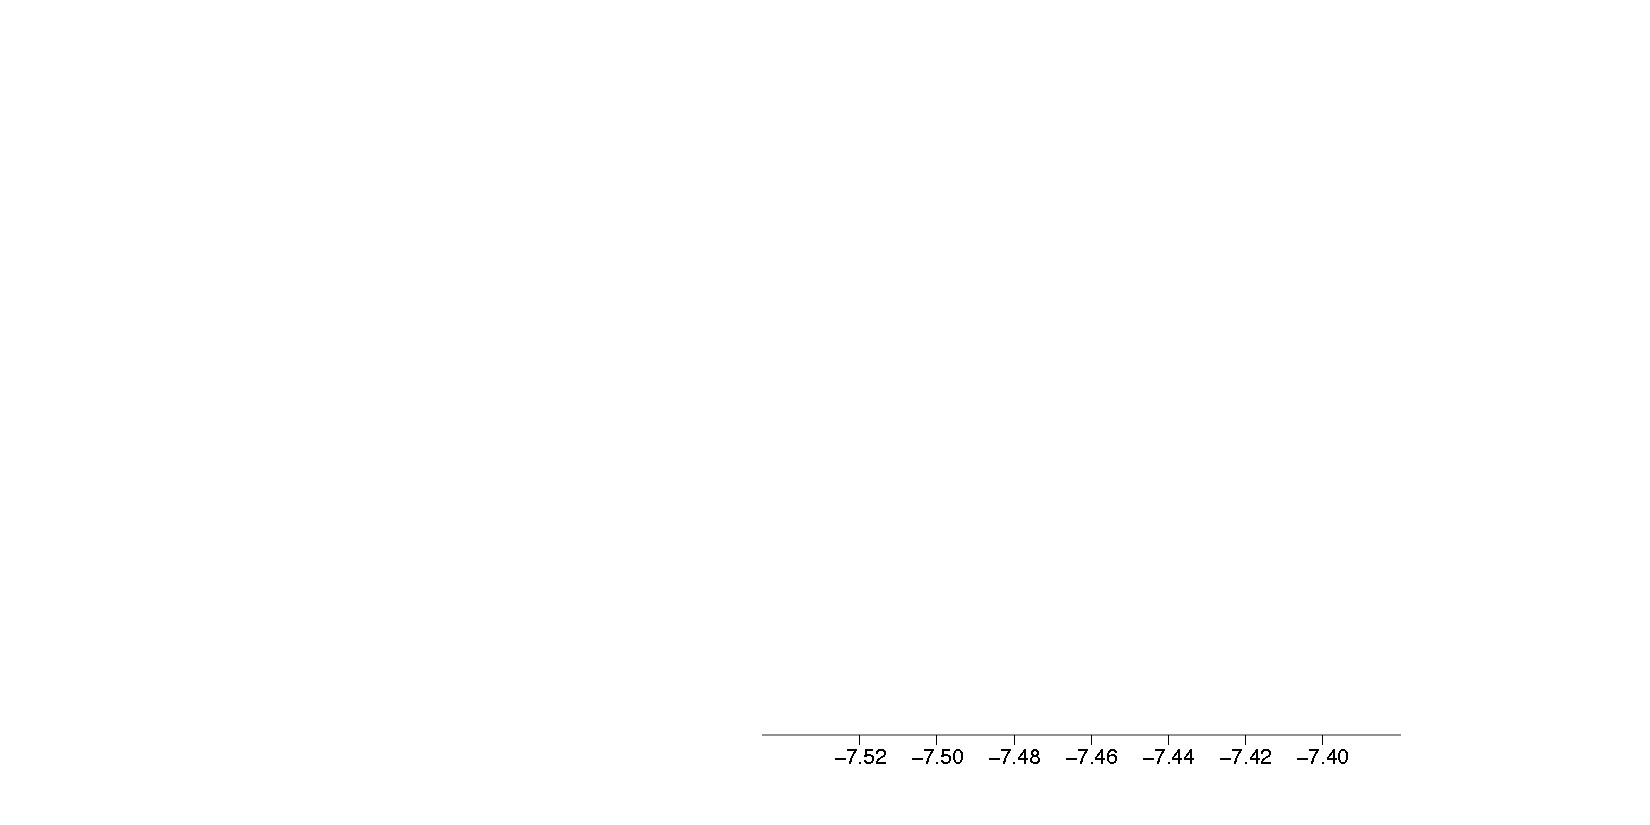
\includegraphics[scale=\graphscale]{reading_tea_leaves/tasks/wiki_x}}
\end{flushright}
\column{.15\linewidth}
  \includegraphics[scale=\graphscale]{reading_tea_leaves/tasks/legend}
\end{columns}
\vspace{-0.75cm}
\begin{center}
  \includegraphics[scale=\graphscale]{reading_tea_leaves/tasks/held-out} \\
\only<1> {within a model, higher likelihood $\not =$ higher interpretability}
\only<2> {across models, higher likelihood $\not =$ higher interpretability}
\end{center}
}


\begin{frame}
  \frametitle{Evaluation Takeaway}

  \begin{itemize}
    \item Measure what you care about~\cite{chang-09c}
      \item If you care about prediction, likelihood is good
\item If you care about a particular task, measure that
    \end{itemize}

\end{frame}

\fi


\begin{frame}
  \frametitle{Outline of This Talk}

  \begin{columns}
    \column{.2\linewidth}
       \includegraphics[width=\linewidth]{cognitive/crowdsourcing_on}
    \column{.6\linewidth}
       \begin{block}{Evaluating Topic Models}
         Crowdsourced evaluation of topic models
        \end{block}

  \end{columns}


  \begin{columns}
    \column{.2\linewidth}
       \includegraphics[width=\linewidth]{cognitive/user_on}
    \column{.6\linewidth}
       \begin{block}{Interaction}
         Representing meaning and new applications
        \end{block}

  \end{columns}


  \begin{columns}
    \column{.2\linewidth}
       \includegraphics[width=\linewidth]{cognitive/algorithms_on}
    \column{.6\linewidth}
       \begin{block}{Algorithms}
         Efficient algorithms for streaming datasets
        \end{block}
  \end{columns}

  \begin{columns}
    \column{.2\linewidth}
       \includegraphics[width=\linewidth]{cognitive/framing_on}
    \column{.6\linewidth}
       \begin{block}{Computational Social Science}
         Detecting spin via hierarchical models
        \end{block}

  \end{columns}

\end{frame}

\section{Evaluating Topic Models}

\begin{frame}
  \vspace{-2cm}
  \begin{columns}
    \column{.45\linewidth}
    \begin{center}
      \includegraphics[width=\linewidth]{cognitive/crowdsourcing_on}
      \end{center}
    \column{.45\linewidth}
    \begin{center}
      \includegraphics[width=\linewidth]{cognitive/user_off}
      \end{center}

  \end{columns}

  \begin{columns}
    \column{.45\linewidth}
    \begin{center}
      \includegraphics[width=\linewidth]{cognitive/algorithms_off}
      \end{center}
    \column{.45\linewidth}
    \begin{center}
      \includegraphics[width=\linewidth]{cognitive/framing_off}
      \end{center}
  \end{columns}

\only<2->{
\vspace{-3cm}
\begin{block}{Reading Tea Leaves}
        How we used to evaluate topic models was wrong; but there is a better
        way using crowdsourcing
\end{block}
}

\end{frame}

\begin{frame}{Evaluating Topic Models}

\begin{columns}

\column{.6\linewidth}
\begin{block}{ Reading Tea Leaves: How Humans Interpret Topic Models}
Jonathan Chang, Jordan Boyd-Graber, Chong Wang, Sean Gerrish, and David
M. Blei. Reading Tea Leaves: How Humans Interpret Topic Models. Neural
Information Processing Systems, 2009.
\end{block}

{\bf Jonathan and I shared a NIPS 2009 Best Student Paper HM}

\column{.3\linewidth}
\includegraphics[width=.8\linewidth]{general_figures/jonathan}

\end{columns}

\end{frame}



\frame{
\frametitle{Evaluation}
\begin{center}
%\only<1>{\includegraphics[width=0.9\linewidth]{reading_tea_leaves/figures/heldout_1} }
\only<1>{\includegraphics[width=\linewidth]{reading_tea_leaves/figures/heldout_2} }
%\only<3>{\includegraphics[width=\linewidth]{reading_tea_leaves/figures/heldout_3} }
\only<2>{\includegraphics[width=\linewidth]{reading_tea_leaves/figures/heldout_4}  \\
	\large Measures predictive power (likelihood / perplexity)}
\end{center}
}


\frame{
        \frametitle{Interruption}

  \begin{columns}
  \column{.6\linewidth}
  \begin{block}{Do you have any real results?}
  \centering
     \includegraphics[width=0.5\linewidth]{reading_tea_leaves/jelinek} \\
     Fred Jelinek, inventor of perplexity~\cite{jelinek-76}
  \end{block}

  \column{.4\linewidth}

  \begin{itemize}
    \item Computational linguists and machine learning researchers like {\bf numbers}
    \item Likelihood and perplexity are convenient numbers
    \pause
    \item What do we {\bf actually} care about in topic models?
  \end{itemize}

  \end{columns}
}

\frame{
\frametitle{Qualitative Evaluation of the Latent Space}

\begin{center}
\only<1>{\includegraphics[width=0.9\linewidth]{reading_tea_leaves/topics_from_papers/1} \\ \cite{hofmann-99} }
\only<2>{\includegraphics[width=0.7\linewidth]{reading_tea_leaves/topics_from_papers/2} \\ \cite{blei-03} }
\only<3>{\includegraphics[width=0.7\linewidth]{reading_tea_leaves/topics_from_papers/3} \\ \cite{mimno-09} }
\only<4>{\includegraphics[width=0.7\linewidth]{reading_tea_leaves/topics_from_papers/4} \\ \cite{maskeri-08} }

\only<5->{
\begin{block}{Interpretability}
        When a user looks at a topic, does it make sense?
\end{block}
\pause
  \begin{itemize}
   \item Interpretability is a human judgment
    \item We will ask people directly
    \item Experiment Goals
      \begin{itemize}
        \item Quick
        \item Fun
        \item Consistent
      \end{itemize}
      \pause
      \item We turn to Amazon Mechanical Turk
        \iflong
       \item Two tasks: Word Intrusion and Topic Intrusion
         \else
         \item Primary task: Word Intrusion
         \fi

  \end{itemize}
}
\end{center}
}

\frame{
\frametitle{Data from the Cloud}
\begin{columns}[c]


\column{0.45\linewidth}

\begin{block}{Then}
\includegraphics[width=0.95\linewidth]{evocation/figures/mechanical_turk_old}
\end{block}


\column{0.45\linewidth}

\begin{block}{Now}
\includegraphics[width=0.95\linewidth]{evocation/figures/mechanical_turk_new}
\end{block}

\end{columns}
}

\frame{
  \frametitle{Word Intrusion}

  \begin{enumerate}
    \item Take the highest probability words from a topic

      \begin{block}{Original Topic}
        dog, cat, horse, pig, cow
      \end{block}
\pause
    \item Take a high-probability word from another topic and add it
      \begin{block}{Topic with Intruder}
        dog, cat, \alert<2->{apple}, horse, pig, cow
      \end{block}
\pause
     \item We ask users to find the word that doesn't belong
  \end{enumerate}
\begin{block}{Hypothesis}
If the topics are interpretable, users will consistently choose true intruder
\end{block}
}

\frame{
  \frametitle{Word Intrusion}

\begin{center}
\only<1>{\includegraphics[width=\linewidth]{reading_tea_leaves/tasks/word1}  }
\only<2>{\includegraphics[width=\linewidth]{reading_tea_leaves/tasks/word2}  }
\pause
  \begin{itemize}
    \item Order of words was shuffled
    \item Which intruder was selected varied
    \item Model precision: percentage of users who clicked on intruder
  \end{itemize}

\end{center}
}


\frame{
\frametitle{Word Intrusion: Which Topics are Interpretable?}
  \begin{block}{New York Times, 50 Topics}
    \begin{center}
      \includegraphics[width=0.8\linewidth]{reading_tea_leaves/figures/topic_precision}
    \end{center}
  \end{block}
  \begin{center}
    Model Precision: percentage of correct intruders found
  \end{center}
}

\frame{

\frametitle{Interpretability and Likelihood}

\begin{center}
\only<1>{Model Precision on New York Times}
\end{center}

\begin{columns}
\column{.84\linewidth}
\begin{flushright}
  \only<1>{\includegraphics[scale=\graphscale]{reading_tea_leaves/tasks/mp}}
  \only<1>{\includegraphics[scale=\graphscale]{reading_tea_leaves/tasks/mp_y}\includegraphics[scale=\graphscale]{reading_tea_leaves/tasks/nyt_mp}\\}
  \only<1>{\includegraphics[scale=\graphscale]{reading_tea_leaves/tasks/nyt_x}}

\end{flushright}
\column{.15\linewidth}
  \includegraphics[scale=\graphscale]{reading_tea_leaves/tasks/legend}
\end{columns}
\vspace{-0.75cm}
\begin{center}
  \includegraphics[scale=\graphscale]{reading_tea_leaves/tasks/held-out} \\
\only<1> {within a model, higher likelihood $\not =$ higher interpretability}
\end{center}
}


\begin{frame}{Since then \dots}

  \begin{itemize}
    \item A way to get at an evaluation that matches {\bf what we care about}
    \item A necessary step to improving topic models for navigating large datasets~\cite{talley-11}
    \item Others have discovered automatic methods that uncover the same properties~\cite{newman-10,mimno-11}
    \item And extended the technique to structured topics and phrases~\cite{lindsey-12,weninger-12}
  \end{itemize}

\end{frame}

\section{Interactive Topic Modeling}

\begin{frame}
  \vspace{-2cm}
  \begin{columns}
    \column{.45\linewidth}
    \begin{center}
      \includegraphics[width=\linewidth]{cognitive/crowdsourcing_off}
      \end{center}
    \column{.45\linewidth}
    \begin{center}
      \includegraphics[width=\linewidth]{cognitive/user_on}
      \end{center}

  \end{columns}

  \begin{columns}
    \column{.45\linewidth}
    \begin{center}
      \includegraphics[width=\linewidth]{cognitive/algorithms_off}
      \end{center}
    \column{.45\linewidth}
    \begin{center}
      \includegraphics[width=\linewidth]{cognitive/framing_off}
      \end{center}
  \end{columns}

\only<2->{
\vspace{-3cm}
\begin{block}{Interactive Topic Modeling}
        When a topic model goes bad, a novice user can fix it.
\end{block}
}

\end{frame}


\frame{

\begin{columns}

\column{.5\linewidth}

\includegraphics[width=.8\linewidth]{general_figures/yuening}

\column{.5\linewidth}

\begin{block}{Interactive Topic Modeling}
Yuening Hu, Jordan Boyd-Graber, Brianna Satinoff, and Alison Smith. Interactive Topic Modeling. Machine Learning, 2014.
\end{block}

\end{columns}

}


\frame{

\frametitle{The Problem: User Perspective}

\begin{columns}

\column{.4\linewidth}
\begin{center}
\begin{tabular}{ccc}
& \only<2->{\itmspace}\color<2->{red}{bladder} & \\
& \only<3->{\hspace{-2cm}} \color<3->{blue}{spinal\_cord}  & \\
& \only<3->{\hspace{-2cm}} \color<3->{blue}{sci} & \\
& \only<3->{\hspace{-2cm}}\color<3->{blue}{spinal\_cord\_injury} & \\
& \only<3->{\hspace{-2cm}}\color<3->{blue}{spinal} & \\
& \only<2->{\itmspace}\color<2->{red}{urinary} & \\
& \only<2->{\itmspace}\color<2->{red}{urothelial} & \\
& \only<3->{\hspace{-2cm}}\color<3->{blue}{cervical} & \\
& injury & \\
& recovery & \\
& \only<2->{\itmspace}\color<2->{red}{urinary\_tract} & \\
& locomotor & \\
& \only<3->{\hspace{-2cm}}\color<3->{blue}{lumbar} & \\
\end{tabular}
\end{center}

\column{.6\linewidth}

\danquote{These words don't belong together!}

\end{columns}

}

\begin{frame}
        \frametitle{This is serious business!}


        \begin{itemize}
          \item Decision makers see problems
          \item No easy way to correct the problem
          \item Result: entire approach is abandoned
\pause
          \item Two ingredients in the fix:
            \begin{itemize}
              \item New models
              \item How to learn from mistakes
            \end{itemize}
        \end{itemize}

\end{frame}



\frame{
	\frametitle{Fix Ingredient \#1: The model}

\begin{columns}

\column{.4\linewidth}

\begin{itemize}
	\item The topics in a topic model are \only<2->{\alert<2>{uncorrelated}} distributions over words
	\only<3->{
	\item The advice you get can be encoded as correlations
		\begin{itemize}
			\alert<4>{\item Positive correlations}
			\alert<5>{\item Negative correlations}
		\end{itemize}
	}

\end{itemize}

\column{.6\linewidth}

	\only<1-2>{	\includegraphics[width=\linewidth]{interactive_topic_models/constraints_1}     }
	\only<3-4>{	\includegraphics[width=\linewidth]{interactive_topic_models/constraints_2}     }
	\only<5->{	\includegraphics[width=\linewidth]{interactive_topic_models/constraints_3}     }
\end{columns}

}

\begin{frame}
  \frametitle{Adding meaning to topic models}

        \begin{itemize}
	 \item Add an additional step to model topics as a distribution over concepts

         \item We've used this formalism to build probabilistic word-sense
           disambiguation algorithms~\cite{boyd-graber-07} and multilingual models~\cite{boyd-graber-10}

         \item Others have used it to encode database constraints (e.g. cannot link and must link)~\cite{andrzejewski-09} or first order logic~\cite{andrzejewski-11}
        \end{itemize}

\end{frame}

\begin{frame}
  \frametitle{Adding meaning to topic models}
        \begin{block}{Traditional Topic Models}
                $ p(w) = \prod_d \prod_n^{N_d} \left( p(w_{d,n} | \phi_{z_{d,n}})
                  \explain{\alert<3>{topic}}{p(z_{d,n} | \theta_d)} \right) p(\theta_d | \alpha)                 \explain{\alert<2>{topic to words}}{ \prod_k^K
p(\phi_k | \eta) }$
        \end{block}

        \begin{block}{Our Model}
          \vspace{-0.8cm}
          \begin{align*}
               p(w) = \prod_d \prod_n^{N_d} & \left( p(w_{d,n} | \pi_{l_{d,n}})
                 \explain{\alert<6>{meaning and topic}} {p(l_{d,n} | \phi_{d,n} )
                   p(z_{d,n} | \theta_d)}  \right) p(\theta_d | \alpha) \\
               &  \explain{\alert<4>{topic to concept}}{\prod_k^K
                p(\phi_k | \eta)} \explain{\alert<5>{concept to word}}{\prod_c^C \left(
                  p(\pi_{k,c} | \tau) \right) }
           \end{align*}
        \end{block}


\end{frame}

\begin{frame}

        % TODO(jbg): add image
        \frametitle{Fix Ingredient \#2: Online Learning}

        \begin{itemize}
                \item Feedback shows data where you made mistakes
                \item ``Forget'' those data~\cite{yao-09}
                \item Then rerun inference, pretending you're seeing them for the first time
                \item Allows you to escape from local optima
        \end{itemize}

\end{frame}


\frame{
	\frametitle{How to incorporate feedback?}

	\begin{columns}

	\column{.5\linewidth}

		\begin{columns}

			\column{.6\linewidth}

			\includegraphics[width=\linewidth]{topic_models/nyt_topics}


			\column{.4\linewidth}
			\begin{center}
				\only<2->{\includegraphics[width=.6\linewidth]{general_figures/arrow_right_down} \\}
				\only<2->{\includegraphics[width=.6\linewidth]{general_figures/milkman_dan} \\}
				\invisible<-2>{\includegraphics[width=.6\linewidth,angle=270]{general_figures/arrow_right_down}}
			\end{center}

		\end{columns}

	\column{.5\linewidth}

	\begin{enumerate}
		\item Fit initial topic model
			\pause
		\item Get feedback from user
			\pause
		\item Incrementally relearn model
			\begin{itemize}
                                \item Forget your mistakes
				\item Replace the model with a correlated one
				\item Continue inference
			\end{itemize}
	\end{enumerate}
\pause
Keep computation \alert<4>{fast and consistent} \cite{Hu-12a}
	\end{columns}

}

\providecommand{\tb}[1]{\parbox{0.8\linewidth}{ \tiny{ #1 }} \vspace{.2cm} }

\frame{

\vspace{-1cm}

\begin{columns}

\column{.5\linewidth}

\begin{tabular}{l*{2}{c}r}
	Topic & Before \\
\hline

\alert<2>{{\bf 1}} & \tb{ \alert<2>{election, yeltsin, russian, political, party, democratic, russia,
  president, democracy, boris, country, south, years, month, government, vote,
  since, leader, presidential, military} } \\

2 & \tb{new, york, city, state, mayor, budget, giuliani, council, cuomo, gov,
  plan, year, rudolph, dinkins, lead, need, governor, legislature, pataki,
  david} \\

3 & \tb{nuclear, arms, weapon, defense, treaty, missile, world, unite, yet,
  soviet, lead, secretary, would, control, korea, intelligence, test, nation,
  country, testing} \\

4 & \tb{president, bush, administration, clinton, american, force, reagan, war,
  unite, lead, economic, iraq, congress, america, iraqi, policy, aid,
  international, military, see} \\

& \vdots \\

\alert<2>{{\bf 20}} & \tb{\alert<2>{soviet, lead, gorbachev, union, west, mikhail, reform, change, europe,
  leaders, poland, communist, know, old, right, human, washington, western,
  bring, party} }\\

\end{tabular}

\column{.5\linewidth}

\only<3> {

	\begin{block}{Suggestion}
	\emph{boris, communist, gorbachev, mikhail, russia,
  russian, soviet, union, yeltsin }
	\end{block}

}

\only<4-> {

\begin{tabular}{l*{2}{c}r}
	Topic & After \\
\hline

\alert<5>{{\bf 1}} & \alert<5>{\tb{election, democratic, south, country, president, party, africa, lead,
  even, democracy, leader, presidential, week, politics, minister, percent,
  voter, last, month, years} } \\

\alert<6>{2} & \tb{new, york, city, state, mayor, budget, council, giuliani, gov, cuomo,
  year, rudolph, dinkins, legislature, plan, david, governor, pataki, need, cut}
\\

\alert<6>{3} & \tb{nuclear, arms, weapon, treaty, defense, war, missile, may, come, test,
  american, world, would, need, lead, get, join, yet, clinton, nation} \\

\alert<6>{4} & \tb{president, administration, bush, clinton, war, unite, force, reagan,
  american, america, make, nation, military, iraq, iraqi, troops, international,
  country, yesterday, plan} \\

   & \vdots \\

\alert<4>{ {\bf 20} } & \alert<4> {\tb{soviet, union, economic, reform, yeltsin, russian, lead, russia,
  gorbachev, leaders, west, president, boris, moscow, europe, poland, mikhail,
  communist, power, relations} } \\

\end{tabular}

}

\end{columns}

}


\providecommand{\blue}[1]{{\color{blue}{#1}}}
\providecommand{\red}[1]{{\color{red}{#1}}}
\providecommand{\green}[1]{{\color{green}{#1}}}

\begin{frame}

\frametitle{Example: Negative Constraint}

\begin{columns}

\column{.4\linewidth}

\begin{tabular}{l*{2}{c}r}
	Topic & Words \\
\hline

{\bf 318} & \tb{\red{bladder}, sci, \blue{spinal\_cord}, \blue{spinal\_cord\_injury}, \blue{spinal}, \red{urinary}, \red{urinary\_tract}, \red{urothelial},\blue{injury}, \blue{motor}, \blue{recovery}, \blue{reflex}, \blue{cervical}, \red{urothelium}, \blue{functional\_recovery}} \\

\end{tabular}

\column{.1\linewidth}

\column{.4\linewidth}

\only<3->{
\begin{tabular}{l*{2}{c}r}
	Topic & Words \\
\hline

{\bf 318} & \tb{sci, \blue{spinal\_cord}, \blue{spinal\_cord\_injury}, \blue{spinal}, \blue{injury}, \blue{recovery}, \blue{motor}, \blue{reflex}, \red{urothelial}, \green{injured}, \blue{functional\_recovery}, \green{plasticity}, \green{locomotor}, \blue{cervical}, \green{locomotion}}\\

\end{tabular}
}

\end{columns}

\only<2->{
\begin{block}{Negative Constraint}
  spinal\_cord, bladder
\end{block}

}

\end{frame}




\begin{frame}

        \frametitle{Experiments}

\begin{columns}

\column{.5\linewidth}

  \begin{itemize}
   \item Simulating users through classifying social media
     \begin{itemize}
       \item Investigating different learning strategies
       \item How much to forget
     \end{itemize}
   \end{itemize}

\column{.5\linewidth}

\begin{center}
\includegraphics[width=\linewidth]{interactive_topic_models/ablation_30_topics}
\end{center}

\end{columns}

\begin{itemize}
    \item User study: mechanical Turk
      \begin{itemize}
        \item We can't do everything users want: proper names, mac vs. pc
        \item Users are senstive to polysemy (``msg'': food or e-mail)
      \end{itemize}
    \item User study: exploring congressional debates
      \begin{itemize}
        \item Collaboration with social scientists
        \item Interactivity makes people use topic models more
       \end{itemize}
  \end{itemize}


\end{frame}

\section{Real-Word Evaluation}

\frame{

\begin{columns}

\column{.5\linewidth}

\includegraphics[width=.8\linewidth]{general_figures/forough}

\column{.5\linewidth}

\begin{block}{ALTO: Active Learning with Topic Overviews for Speeding Label Induction and Document Labeling}
Forough Poursabzi-Sangdeh, Jordan Boyd-Graber, Leah Findlater, and Kevin Seppi.  Association for Computational Linguistics, 2016.
\end{block}

\end{columns}

}

\fsi{interactive_topic_models/messy-desk}{Many Documents}

\fsi{interactive_topic_models/file-cabinet}{Sort into Categories}

\begin{frame}{Evaluation}

  \begin{itemize}
    \item User study
    \item 40 minutes
    \item Sort documents into categories
    \item What information / interface \alert<2>{helps best}
      \pause
      \pause
      \begin{itemize}
        \item Train a classifier on human examples
          \only<4->{\alert<4>{(don't tell them how many labels)}}
        \item Compare classifier labels to expert judgements
          \only<5->{\alert<5>{(purity)}}
\only<5>{
\begin{equation}
\mbox{purity}(\mathbf{U},\mathbf{G}) = \frac{1}{N}\sum\limits_{l} \max\limits_{j}|U_l \cap G_j|,
\end{equation}
}
      \end{itemize}
  \end{itemize}

\end{frame}

\begin{frame}{Which is more Useful?}

\only<1>{
  \begin{center}
    Who should drive?
  \end{center}
}


\only<2->{
\begin{columns}
  \column{.5\linewidth}
    \begin{block}{Active Learning}
      \begin{center}
        \includegraphics[width=.85\linewidth]{interactive_topic_models/active_learning}
      \end{center}
    \end{block}
  \column{.5\linewidth}
  \pause
    \begin{block}{Topic Models}
      \begin{center}
        \includegraphics[width=.475\linewidth]{interactive_topic_models/nyt_topics}
      \end{center}

    \end{block}


\end{columns}
}

\end{frame}

\fsi{interactive_topic_models/alto_interface}{}
\fsi{interactive_topic_models/alto_interface_highlight}{Direct users
  to document}



\fsi{interactive_topic_models/alto/user_talk_1}{ Active learning if time is short}
\fsi{interactive_topic_models/alto/user_talk_2}{ Better than status quo}
\fsi{interactive_topic_models/alto/user_talk_3}{ Active learning can
  help topic models }
\fsi{interactive_topic_models/alto/user_talk_4}{ Topic models help
  users understand the collection }
\fsi{interactive_topic_models/alto/user_talk_4}{ Moral: machines and
  humans together (if you let them) }

\begin{frame}{Real-World Use Cases}

\begin{columns}
  \column{.3\linewidth}
  \includegraphics[width=\linewidth]{topic_models/fcc-logo}
  \column{.3\linewidth}
  \includegraphics[width=\linewidth]{topic_models/gsa}
  \column{.3\linewidth}
  \includegraphics[width=\linewidth]{general_figures/nsf}
\end{columns}

\begin{center}
  \includegraphics[width=.4\linewidth]{interactive_topic_models/disaster}
\end{center}

\end{frame}


\section{Online LDA With Infinite Vocabulary}

\begin{frame}
  \vspace{-2cm}
  \begin{columns}
    \column{.45\linewidth}
    \begin{center}
      \includegraphics[width=\linewidth]{cognitive/crowdsourcing_off}
      \end{center}
    \column{.45\linewidth}
    \begin{center}
      \includegraphics[width=\linewidth]{cognitive/user_off}
      \end{center}

  \end{columns}

  \begin{columns}
    \column{.45\linewidth}
    \begin{center}
      \includegraphics[width=\linewidth]{cognitive/algorithms_on}
      \end{center}
    \column{.45\linewidth}
    \begin{center}
      \includegraphics[width=\linewidth]{cognitive/framing_off}
      \end{center}
  \end{columns}

\only<2->{
\vspace{-3cm}
\begin{block}{Infinite Vocabulary Topic Models}
        A model that can handle big, streaming data without assuming a fixed vocabulary
\end{block}
}


\end{frame}



\frame{

\begin{columns}

\column{.5\linewidth}

\begin{block}{Online Topic Models with Infinite Vocabulary}
Ke Zhai and Jordan Boyd-Graber.  International Conference on Machine Learning, 2013.
\end{block}

\column{.5\linewidth}

\includegraphics[width=.8\linewidth]{general_figures/ke}

\end{columns}

}

\begin{frame}{The Problem}

  \begin{center}
    \includegraphics[width=.7\linewidth]{infvoc/batch} \\
    Batch algorithms can't scale
  \end{center}

\end{frame}

\begin{frame}{One Solution: Parallelization}
  \begin{center}
    \includegraphics[width=.7\linewidth]{infvoc/parallel} \\
    Throw more computers at the problem \\
    For topic models, \textsc{Mr Lda}~\cite{zhai-12}
  \end{center}
\end{frame}

\begin{frame}{Another Solution: Streaming Algorithms}
  \begin{center}
    \only<1>{ \includegraphics[width=.8\linewidth]{infvoc/streaming-0}}
    \only<2>{ \includegraphics[width=.8\linewidth]{infvoc/streaming-1}}
    \only<3>{ \includegraphics[width=.8\linewidth]{infvoc/streaming-2}}
    \only<4>{ \includegraphics[width=.8\linewidth]{infvoc/streaming-3}}
    \only<5>{ \includegraphics[width=.8\linewidth]{infvoc/streaming-4}}
    \only<6>{ \includegraphics[width=.8\linewidth]{infvoc/streaming-5}}
    \only<7>{ \includegraphics[width=.8\linewidth]{infvoc/streaming-6}}
    \only<8>{ \includegraphics[width=.8\linewidth]{infvoc/streaming-7}}
    \\
    Handle the data as they come
  \end{center}
\end{frame}


% Making inference more efficient

% Streaming algorithms

% Why this is a problem for LDA


\begin{frame}{Online Topic Models}

\begin{block}{Past approaches for online topics models}
\begin{itemize}
%\item Gibbs sampling~\cite{yao-09}
\item Sequential Monte Carlo~\cite{canini-09}
%\item With the idea of an evolution matrix~\citep{alsumait-08}
\item Variational inference~\cite{hoffman-10}
\item Hybrid MCMC inference~\cite{mimno-12}
\end{itemize}
\end{block}

\begin{block}{Same assumption: constant vocabulary}
\begin{itemize}
\item The vocabulary is known \textit{a priori}
\item Topic distribution is {\bf fixed} Dirichlet \\
\begin{center}
$\boldsymbol{\beta}_k \sim \dir{\lambda}$.
\end{center}
\end{itemize}
\end{block}

\end{frame}

\begin{frame}{Online Algorithms and Fixed Vocabularies}

\begin{block}{}
\begin{itemize}
\item proper nouns, e.g., ``sch\"{a}uble''
\item words being invented, e.g., ``crowdsourcing''
\item words cross languages, e.g., ``Gangnam''
\item words cross topics, e.g., ``vuvuzelas'' (\textit{music}
  $\rightarrow$ \textit{sports}), etc
\end{itemize}
\end{block}
\pause
\begin{columns}

\column{.5\linewidth}

\centering
\includegraphics[width=.5\linewidth]{infvoc/psy}


\column{.5\linewidth}

\begin{itemize}
  \item Hard-to-detect errors: \{``style'', ``korea'',
    ``download'', ``youtube''\}
\pause
      \item Our approach: an infinite vocabulary
\end{itemize}


\end{columns}

\end{frame}

% Nonparametric models

\begin{frame}{The Infinite Dirichlet Process}
  \only<1>{ \includegraphics[width=.95\linewidth]{infvoc/dp_monkey-1} }
  \only<2>{ \includegraphics[width=.95\linewidth]{infvoc/dp_monkey-2} }
  \only<3>{ \includegraphics[width=.95\linewidth]{infvoc/dp_monkey-3} }
  \only<4>{ \includegraphics[width=.95\linewidth]{infvoc/dp_monkey-5} }
  \only<5>{ \includegraphics[width=.95\linewidth]{infvoc/dp_monkey-6} }
  \only<6>{ \includegraphics[width=.95\linewidth]{infvoc/dp_monkey-7} }
  \only<7>{ \includegraphics[width=.95\linewidth]{infvoc/dp_monkey-8} }
  \only<8>{ \includegraphics[width=.95\linewidth]{infvoc/dp_monkey-9} }
  \only<9>{ \includegraphics[width=.95\linewidth]{infvoc/dp_monkey-10} }
  \only<10->{ \includegraphics[width=.95\linewidth]{infvoc/dp_monkey-11} \\}
  \only<11->{Example of Bayesian nonparametrics \cite{ferguson-73,sethuraman-94}}
\end{frame}

% Our model

\begin{frame}{Infinite Vocabulary Topic Model}

  \begin{columns}
     \column{.44\linewidth}
     \begin{itemize}
       \item Each topic $\theta_k \sim \mbox{DP}(\alpha, G_0)$
       \item Infinite collection of atoms and weights
     \begin{itemize}
       \item For each word, ``stick breaks'' \alert<2>{$b_{k, w} \sim \mbox{Beta}(1,\alpha)$}
       \item Each atom gets weight \alert<3>{$\beta_{k, w} = \prod_{j=1}^{w} (1 - b_j)$}
       \item Atom identity drawn from base distribution $\rho_k \sim G_0$
     \end{itemize}
     \end{itemize}
     \column{.55\linewidth}
       \includegraphics[width=1.0\linewidth]{infvoc/dp_monkey-topics}
  \end{columns}

\end{frame}

% Comics

\begin{frame}{Inference}

We can't optimize the joint likelihood
\begin{align}
& \textstyle p( \boldsymbol{W}, \boldsymbol{\rho}, \boldsymbol{\beta},
\boldsymbol{\theta}, \boldsymbol{z} ) = \prod_{k=1}^K
\left[ \prod_{t=1}^{\infty} p( \rho_{kt} | G_0 ) \cdot p( \beta_{kt}
| \alpha^{\beta} ) \right] \notag \\
& \textstyle \left[ \prod_{d=1}^{D} p( \boldsymbol{\theta}_d | \alpha^{\theta} )
\prod_{n=1}^{N_d} p( z_{dn} | \boldsymbol{\theta}_d ) p( \omega_{dn} |
z_{dn}, \boldsymbol{\beta}_{z_{dn}} ) \right] . \notag
\end{align}
\pause
so we optimize a lower bound of the objective based on a variational distribution $q$,
\begin{align}
\textstyle \log p(\boldsymbol{W}) \geq {\e{q(\boldsymbol{Z})}{\log p(\boldsymbol{W},\boldsymbol{Z})} - \e{q(\boldsymbol{Z})}{q}} = \elbo,
\label{eq:elbo-vague}
\end{align}
which we optimize $\elbo(\boldsymbol{Z})$ using gradient steps.
\end{frame}



\begin{frame}{Incorporating New Words}
%\begin{center}
%\begin{figure}
  \only<1>{\includegraphics[width=\linewidth]{infvoc/new_words_highlight_1}}
  \only<2>{\includegraphics[width=\linewidth]{infvoc/new_words_highlight_2}}
  \only<3>{\includegraphics[width=\linewidth]{infvoc/new_words_highlight_3}}
  \only<4>{\includegraphics[width=\linewidth]{infvoc/new_words_highlight_4}}
  \only<5>{\includegraphics[width=\linewidth]{infvoc/new_words_highlight_5}}
  \only<6>{\includegraphics[width=\linewidth]{infvoc/new_words_highlight_6}}
  \only<7>{\includegraphics[width=\linewidth]{infvoc/new_words_highlight_7}}
  \only<8>{\includegraphics[width=\linewidth]{infvoc/new_words_highlight_8}}
%\end{figure}
%\end{center}
\begin{center}
\vspace{-5mm}
An example topic from \textit{20 newsgroups} under our model.
Numbers preceeding words are ranks in topic.
\end{center}

\end{frame}


\begin{frame}{Do the topics make sense?}

\centering
       \only<1>{\includegraphics[width=1.0\linewidth]{infvoc/coherence_0}}
       \only<2>{\includegraphics[width=1.0\linewidth]{infvoc/coherence_1}}
       \only<3>{\includegraphics[width=1.0\linewidth]{infvoc/coherence_2}}
       \only<4>{\includegraphics[width=1.0\linewidth]{infvoc/coherence_3}}

\begin{columns}
\column{.5\linewidth}
\begin{itemize}
  \item Finite topic models
  \item ``Dynamic'' topic models
\end{itemize}

\column{.5\linewidth}
\begin{itemize}
  \item Hashed vocabulary
  \item Other inference techniques
\end{itemize}
\end{columns}


\end{frame}


% Interpretability results

%
\ifsupershortmlslda

\else

\frame {

\frametitle{Problem}

\begin{itemize}
	\item We have documents in multiple languages
	\item They are annotated with the same {\bf continuous response}
	\begin{itemize}
		\item Rating of a product
		\item Movie review
		\item Percentage of people who retweet a tweet
                \item Percentage of people consider a comment ``extreme''
	\end{itemize}
	\item Can learning a model in multiple languages at once help?

	\pause

	\begin{block}{}
		For languages where you don't have many resources, {\bf yes!}
	\end{block}

\end{itemize}

}

\begin{frame}[t]{Conceptual Approach}

  \only<1>{\includegraphics[width=0.85\linewidth]{mlslda/text_topics_prediction_0}}
  \only<2>{\includegraphics[width=0.85\linewidth]{mlslda/text_topics_prediction_1}}
  \only<3>{\includegraphics[width=0.85\linewidth]{mlslda/text_topics_prediction_2}}
  \only<4>{\includegraphics[width=0.85\linewidth]{mlslda/text_topics_prediction_3}}
  \only<5>{\includegraphics[width=0.85\linewidth]{mlslda/text_topics_prediction_4}}
  \only<6>{\includegraphics[width=0.85\linewidth]{mlslda/text_topics_prediction_5}}
  \only<7>{\includegraphics[width=0.85\linewidth]{mlslda/text_topics_prediction_6}}

  \only<5>{
  	\begin{center}
		Similar to social science methodology LIWC~\cite{pennebaker-99}
	\end{center}
  }

  \only<6>{
    \begin{itemize}
      \item {\bf Assumption:} We can create list counts from documents in any language
      \item {\bf Observation:} Once we have list counts, underlying language doesn't matter
    \end{itemize}
  }

  \only<7>{
  	\begin{block}{}
		\begin{center}
		What if we don't know the lists?
		\end{center}
	\end{block}
  }

\end{frame}

\iftmreview

\begin{frame}{Putting Pieces Together}

	\begin{itemize}
	\item How do we learn the word lists?
	\begin{itemize}
		\invisible<-2>{  \item Topic Models }
	\end{itemize}


	\item How do ensure that the word lists reflect sentiment?
	\begin{itemize}
		\invisible<-3>{  \item Supervised Topic Models }
	\end{itemize}

	\item How do make the word lists make sense across languages?
	\begin{itemize}
		\invisible<-4>{  \item Semantic Resources } \visible<5>{ }
	\end{itemize}
	\end{itemize}
\end{frame}



\providecommand{\graphscale}{0.6}


\newcommand{\dirfunc}[3]{ \frac{ \prod_{#1}^{#2} \g{ #3 } } { \g{ \sum_{#1}^{#2} #3 }}}
\newcommand{\dirnum}[4]{ \frac{\g{ #3 }}{#4} \prod_{#1}^{#2} }
\newcommand{\dirden}[3]{ \g{ \sum_{#1}^{#2} #3 } }

\section{Topic Model Introduction}

\begin{frame}

	\frametitle{Why topic models?}

	\begin{columns}

	\column{.3\linewidth}

	\includegraphics[width=1\linewidth]{topic_models/newspapers}

	\column{.55\linewidth}

	\begin{itemize}
		\item Suppose you have a huge number of documents
		\item Want to know what's going on
		\item Can't read them all (e.g. every New York Times article from the 90's)
		\item Topic models offer a way to get a corpus-level view of major themes
		\pause
		\item Unsupervised
	\end{itemize}


	\end{columns}

\end{frame}

\frame{
\begin{center}
\frametitle{Conceptual Approach}
From an \textbf<1>{input corpus} and number of topics \textbf<1>{$K$} $\rightarrow$ \textbf<2>{words to topics} \\
\only<1>{\includegraphics[width=0.6\linewidth]{reading_tea_leaves/figures/heldout_0} }
\only<2>{\includegraphics[width=0.9\linewidth]{reading_tea_leaves/figures/nyt_topics_wide}}
\end{center}
}

\frame{\frametitle{Conceptual Approach}

\begin{itemize}
\item For each document, what topics are expressed by that document?

\begin{center}
\includegraphics[width=0.9\linewidth]{topic_models/nyt_documents}
\end{center}

\end{itemize}
}

\iflong

\begin{frame}

\frametitle{Topics from \emph{Science}}

\begin{center}
\includegraphics[width=0.8\linewidth]{topic_models/example_topics}
\end{center}

\end{frame}


\begin{frame}

\frametitle{Why should you care?}

\begin{itemize}
\item Neat way to explore / understand corpus collections
\begin{itemize}
	\item E-discovery
	\item Social media
	\item Scientific data
\end{itemize}
\item NLP Applications
\begin{itemize}
   \item POS Tagging~\cite{toutanova-08}
   \item Word Sense Disambiguation~\cite{boyd-graber-07}
   \item Word Sense Induction~\cite{brody-09}
   \item Discourse Segmentation~\cite{purver-06}
\end{itemize}
\item Psychology~\cite{griffiths-07}: word meaning, polysemy
\item Inference is (relatively) simple
\end{itemize}

\end{frame}

\frame
{
  \frametitle{Matrix Factorization Approach}

\begin{center}
\includegraphics[width=0.9\linewidth]{topic_models/factorization.pdf}
\end{center}

\begin{columns}
\column{.5\textwidth}
\begin{block}{}
	\begin{itemize}
		\item[K] Number of topics
		\item[M] Number of documents
		\item[V] Size of vocabulary
	\end{itemize}
\end{block}
\column{.5\textwidth}
\pause
\begin{itemize}
\item If you use singular value decomposition (SVD), this technique is called latent semantic analysis.
\item Popular in information retrieval.
\end{itemize}
\end{columns}

}

\begin{frame}

\frametitle{Alternative: Generative Model}

\begin{itemize}
  \item How your data came to be
  \item Sequence of Probabilistic Steps
  \item Posterior Inference
\end{itemize}

\end{frame}

\begin{frame}
	\frametitle{Multinomial Distribution}

	\begin{itemize}
		\item Distribution over discrete outcomes
		\item Represented by non-negative vector that sums to one
		\item Picture representation
	\begin{center}
\includegraphics[width=0.4\linewidth]{topic_models/multinomial}
	\end{center}
		\pause
		\item Come from a Dirichlet distribution

	\end{itemize}


\end{frame}

\begin{frame}

\frametitle{Dirichlet Distribution}

\begin{center}
\includegraphics[width=0.4\linewidth]{topic_models/equations/dirichlet} \\ \bigskip
\pause
\includegraphics[width=0.6\linewidth]{topic_models/dirichlet_1} \\
\includegraphics[width=0.2\linewidth]{topic_models/equations/dirichlet_params_1} \includegraphics[width=0.2\linewidth]{topic_models/equations/dirichlet_params_2} \includegraphics[width=0.2\linewidth]{topic_models/equations/dirichlet_params_3} \\
\pause
\includegraphics[width=0.6\linewidth]{topic_models/dirichlet_2} \\
\includegraphics[width=0.2\linewidth]{topic_models/equations/dirichlet_params_4} \includegraphics[width=0.2\linewidth]{topic_models/equations/dirichlet_params_5} \includegraphics[width=0.2\linewidth]{topic_models/equations/dirichlet_params_6} \\
\end{center}

\end{frame}

\begin{frame}
\frametitle{Dirichlet Distribution}
\begin{center}
\includegraphics[width=0.5\linewidth]{topic_models/sparsity}
\end{center}
\end{frame}

\fi
\ifconjugacy

\begin{frame}
\frametitle{Dirichlet Distribution}
\begin{itemize}
  \item If ${\bm \phi} \sim \Dir(\alpha)$, ${\bm w} \sim \Mult(\phi)$, and $n_k = |\{ w_i : w_i = k\}|$ then
  \begin{align}
  	p(\phi | \alpha, {\bm w}) & \propto p({\bm w} | \phi) p(\phi | \alpha) \\
	                       & \propto  \prod_{k} \phi^{n_k} \pause  \prod_k { \phi^{\alpha_k - 1}} \\
	                       & \propto \prod_k \phi^{\alpha_k + n_k - 1}
  \end{align}
  \item Conjugacy: this {\bf posterior} has the same form as the {\bf prior}
\end{itemize}
\end{frame}

\fi

\ifhighlevel

\else

\frame
{
  \frametitle{Generative Model Approach}

\begin{center}
\only<1>{ \includegraphics[scale=0.4]{topic_models/lda1.pdf} }
\only<2>{ \includegraphics[scale=0.4]{topic_models/lda2.pdf} }
\only<3>{ \includegraphics[scale=0.4]{topic_models/lda3.pdf} }
\only<4->{ \includegraphics[scale=0.4]{topic_models/lda4.pdf} }
\end{center}

\begin{itemize}
\item<1-> For each topic $k \in \{1, \dots, K\}$, draw a multinomial distribution $\beta_k$ from a Dirichlet distribution with parameter $\lambda$
\item<2-> For each document $d \in \{1, \dots, M\}$, draw a multinomial distribution $\theta_d$ from a Dirichlet distribution with parameter $\alpha$
\item<3-> For each word position $n \in \{1, \dots, N\}$, select a hidden topic $z_n$ from the multinomial distribution parameterized by $\theta$.
\item<4-> Choose the observed word $w_n$ from the distribution $\beta_{z_n}$.
\end{itemize}

\only<5->{We use statistical inference to uncover the most likely unobserved variables given observed data.}
}

\fi

\begin{frame}
\frametitle{Topic Models: What's Important}
\begin{itemize}
\item Topic models \only<2>{(latent variables)}
\begin{itemize}
\ifhighlevel
	\item Topics to words
	\item Documents to topics
\else
	\item Topics to words---multinomial distribution
	\item Documents to topics---multinomial distribution
\fi
\end{itemize}
\item Focus in this talk: statistical methods
  \begin{itemize}
    \item Model: story of how your data came to be
    \item Latent variables: missing pieces of your story
    \item Statistical inference: filling in those missing pieces
  \end{itemize}
\item We use latent Dirichlet allocation (LDA)~\cite{blei-03}, a fully Bayesian
  version of pLSI~\cite{hofmann-99}, probabilistic version of
  LSA~\cite{landauer-97}
\end{itemize}

\end{frame}

\ifevaluation


\frame{
\frametitle{Evaluation}
\begin{center}
%\only<1>{\includegraphics[width=0.9\linewidth]{reading_tea_leaves/figures/heldout_1} }
\only<1>{\includegraphics[width=\linewidth]{reading_tea_leaves/figures/heldout_2} }
%\only<3>{\includegraphics[width=\linewidth]{reading_tea_leaves/figures/heldout_3} }
\only<2>{\includegraphics[width=\linewidth]{reading_tea_leaves/figures/heldout_4}  \\
	\large Measures predictive power, not what the topics are}
\end{center}

\begin{center}
\includegraphics[width=0.5\linewidth]{topic_models/equations/evaluation} \\
How you compute it is important too~\cite{wallach-09b}
\end{center}

}

\frame{
  \frametitle{Word Intrusion}

  \includegraphics[width=\linewidth]{reading_tea_leaves/figures/nyt_topics_wide}
}


\frame{
  \frametitle{Word Intrusion}

  \begin{enumerate}
    \item Take the highest probability words from a topic

      \begin{block}{Original Topic}
        dog, cat, horse, pig, cow
      \end{block}
\pause
    \item Take a high-probability word from another topic and add it
      \begin{block}{Topic with Intruder}
        dog, cat, \alert<2->{apple}, horse, pig, cow
      \end{block}
\pause
     \item We ask users to find the word that doesn't belong
  \end{enumerate}
\begin{block}{Hypothesis}
If the topics are interpretable, users will consistently choose true intruder
\end{block}
}

\frame{
\frametitle{Word Intrusion}
\begin{center}
\only<1>{\includegraphics[width=\linewidth]{reading_tea_leaves/tasks/word1}  }
\only<2>{\includegraphics[width=\linewidth]{reading_tea_leaves/tasks/word2}  }
\pause
  \begin{itemize}
    \item Order of words was shuffled
    \item Which intruder was selected varied
    \item Model precision: percentage of users who clicked on intruder
  \end{itemize}

\end{center}
}

\frame{
\frametitle{Word Intrusion: Which Topics are Interpretable?}
  \begin{block}{New York Times, 50 LDA Topics}
    \begin{center}
      \includegraphics[width=0.8\linewidth]{reading_tea_leaves/figures/topic_precision}
    \end{center}
  \end{block}
  \begin{center}
    Model Precision: percentage of correct intruders found
  \end{center}
}



\frame{

\frametitle{Interpretability and Likelihood}
\begin{center}
\only<1>{Model Precision on New York Times}
\only<2>{Topic Log Odds on Wikipedia}
\end{center}

\begin{columns}
\column{.85\linewidth}
\begin{flushright}
  \only<1>{\includegraphics[scale=\graphscale]{reading_tea_leaves/tasks/mp}}
  \only<2>{\includegraphics[scale=\graphscale]{reading_tea_leaves/tasks/tlo}}
  \only<1>{\includegraphics[scale=\graphscale]{reading_tea_leaves/tasks/mp_y}\includegraphics[scale=\graphscale]{reading_tea_leaves/tasks/nyt_mp}}
  \only<2>{\includegraphics[scale=\graphscale]{reading_tea_leaves/tasks/tlo_y}\includegraphics[scale=\graphscale]{reading_tea_leaves/tasks/wiki_tlo}} \\
  \only<1>{\includegraphics[scale=\graphscale]{reading_tea_leaves/tasks/nyt_x}}
  \only<2>{\includegraphics[scale=\graphscale]{reading_tea_leaves/tasks/wiki_x}}
\end{flushright}
\column{.15\linewidth}
  \includegraphics[scale=\graphscale]{reading_tea_leaves/tasks/legend}
\end{columns}
\vspace{-0.75cm}
\begin{center}
  \includegraphics[scale=\graphscale]{reading_tea_leaves/tasks/held-out} \\
\only<1> {within a model, higher likelihood $\not =$ higher interpretability}
\only<2> {across models, higher likelihood $\not =$ higher interpretability}
\end{center}
}


\begin{frame}
  \frametitle{Evaluation Takeaway}

  \begin{itemize}
    \item Measure what you care about~\cite{chang-09c}
      \item If you care about prediction, likelihood is good
\item If you care about a particular task, measure that
    \end{itemize}

\end{frame}

\fi



\fi

\ifhighlevel

\else

\frame{
	\frametitle{Foundation: sLDA}

	\begin{columns}
		\column{.5\linewidth}
		   \includegraphics[width=1\linewidth]{mlslda/slda}
			\begin{center}
			supervised latent Dirichlet allocation \cite{blei-07b}
			\end{center}
		\column{.5\linewidth}
		  \begin{block}{Generative Process}
	\begin{enumerate}
		\item For document $d = 1 \dots D$:
		\begin{enumerate}
			\item Draw distribution over topics $\theta_d \sim \mbox{Dir}(\alpha)$
			\item For each word $n = 1 \dots d_n$
				\begin{enumerate}
					\item Draw a topic list assignment	$z_{d,n} \sim \mbox{Discrete}(\theta_d)$
					\item Draw word $w_{d,n}$ from topic list distribution $w_{d,n} \sim \mbox{Discrete}(\beta_{z_{d,n}})$
				\end{enumerate}
			\item Draw response $y_d \sim \mbox{Norm}(\eta^{\top} \bar{z}, \sigma^2)$
		\end{enumerate}
	\end{enumerate}


		  \end{block}
	\end{columns}

	\begin{center}
Topic lists $\beta$, topic assignments $z$, regression parameters $\eta$ learned via posterior inference
	\end{center}
}

\fi

\begin{frame}{Foundation: SLDA}

  Supervised Latent Dirichlet Allocation~\cite{blei-07b}

	\begin{block}{Scoring a Document}
		\begin{itemize}
			\item Each topic has a score
			\item Each word has a topic
			\item Document score is the average of all word scores
		\end{itemize}
	\end{block}

	\begin{center}
	\includegraphics[width=.9\linewidth]{mlslda/slda_example}
	\end{center}

\end{frame}

\frame{
	\frametitle{How to make this multilingual}

	\begin{itemize}
		\item Topic lists provide a layer of abstraction
		\pause
		\item \dots if word lists are consistent across languages
		\item {\bf Holistic}: no component is learned in isolation
	\end{itemize}

	\pause

\begin{center}
\includegraphics[width=0.6\linewidth]{mlslda/connections}
\end{center}


}

\section{Key Technical Challenge: Correlations Across Languages}



\ifhighlevel

\begin{frame}{Encoding Correlations}

  \begin{itemize}
    \item Statistical NLP typically uses Dirichlet distributions because of conjugacy
   \item Parameter of Dirichlet encode mean and variance
    \pause
    \item But we want correlations!
      \end{itemize}

\begin{center}
  \includegraphics[width=0.85\linewidth]{mlslda/correlations_3}
\end{center}

\end{frame}

\else

\frame {
  \frametitle{Encoding Correlations}

  \begin{itemize}
    \item Statistical NLP typically uses Dirichlet distributions because of conjugacy
    \begin{center}
    	\includegraphics[width=0.5\linewidth]{topic_models/dirichlet_1} \\
    	\includegraphics[width=0.5\linewidth]{topic_models/dirichlet_2}
    \end{center}

    \item Parameter of Dirichlet encode mean and variance
    \pause
    \item But we want correlations!

        \end{itemize}
    \begin{block}{}
    \begin{center}
    \begin{tabular}{ccc}
    	gut & h\v{a}o & good \\
    \end{tabular}
    \end{center}
    \end{block}


}

\frame{
	\frametitle{Encoding Correlations}

\begin{center}
\only<1>{\includegraphics[width=0.85\linewidth]{mlslda/correlations_naive}}
\only<2>{\includegraphics[width=0.85\linewidth]{mlslda/correlations_naive_1}}
\only<3>{\includegraphics[width=0.85\linewidth]{mlslda/correlations_naive_2}}
\only<4>{\includegraphics[width=0.85\linewidth]{mlslda/correlations}}
\only<5>{\includegraphics[width=0.85\linewidth]{mlslda/correlations_1}}
\only<6>{\includegraphics[width=0.85\linewidth]{mlslda/correlations_2}}
\only<7>{\includegraphics[width=0.85\linewidth]{mlslda/correlations_3}}
\end{center}
}

\fi

\section{Sources of Correlation}

\frame
{
  \frametitle{Dictionary}

\begin{columns}
\column{.6\textwidth}

\begin{center}
\includegraphics[width=0.9\linewidth]{mlslda/dictionary}
\end{center}

\column{.4\textwidth}
\begin{block}{}
	\begin{itemize}
		\item CEDICT (Chinese/English) \cite{cedict}
		\item HanDeDict (Chinese/German) \cite{handedict}
		\item Ding (German/English) \cite{richter-08}
	\end{itemize}
\end{block}

\end{columns}

}

\fi

\frame
{
  \frametitle{Multilingual Ontology}

\begin{center}
\includegraphics[width=0.75\linewidth]{mlslda/germanet}
\end{center}

\vspace{-.8cm}

\begin{center}
	\item GermaNet~\cite{hamp-97,kunze-02}
\end{center}

}

%\section{Multilingual Supervised Latent Dirichlet Allocation}

\ifhighlevel

\else

\frame
{
  \frametitle{Generative Model}

\begin{columns}

\column{.4\textwidth}

\begin{block}{}
\begin{enumerate}
	\item For each topic $k = 1 \dots K$, \alert<2>{draw correlated multilingual word distribution $\{{\bm \beta}_k, {\bm \omega}_k, {\bm \phi}_k\}$}
	\item For each document $d$, $\theta_d \sim \mbox{Dir}(\alpha)$
	\begin{enumerate}
	\item $z_{d,n} \sim \mbox{Discrete}(\theta_d)$
	\item \alert<3> {Draw path $\lambda_{d,n}$ through multilingual tree $z_{d,n}$, emit $w_{d,n}$}
	\end{enumerate}
	\item $y_d \sim \mbox{Norm}(\eta^{\top} \bar{z}, \sigma^2)$
\end{enumerate}
\end{block}

\column{.6\textwidth}

\begin{center}
\includegraphics[width=0.9\linewidth]{mlslda/mlslda}
\end{center}

\end{columns}

}

\fi

\iflong

\frame{
	\frametitle{Inference}

	\begin{itemize}
		\item Jointly sample $z$ and path $\lambda$ through multilingual tree

\begin{align}
\textstyle
p(&z_{n} = k, \lambda_{n} = r | {\bm z}_{-n}, {\bm \lambda}_{-n}, w_n, \eta, \sigma, \Theta) = \nonumber \\
& p(y_d | {\bm z}, \eta, \sigma) p(\lambda_{n} = r | z_{n} = k, {\bm \lambda}_{-n}, w_n, {\bm \tau}, {\bm \kappa}, {\bm \pi}) \nonumber \\
& p(z_{n} = k | {\bm z}_{-n}, \alpha). \nonumber
\label{eq:path-topic-sampling}
\end{align}

		\item Collapse out multinomial distributions in tree
		\item Slice sample hyperparameters
		\item After pass of $z$, update $\eta$
	\end{itemize}
}

\fi

\ifsupershortmlslda

\frame{
\frametitle{Multilingual Supervised LDA}
\begin{center}
\includegraphics[width=0.9\linewidth]{mlslda/german_amazon_dict}
\end{center}
}

\else

\begin{comment}
\column{.3\textwidth}
\begin{block}{}
	\begin{enumerate}
		\item For each topic 1 \dots K, draw correlated multilingual word distribution $\{\beta, \omega, \phi\}$
		\item For each document in language:
		\begin{enumerate}
			\item Draw distribution over topics $\theta_d \sim \mbox{Dir}(\alpha)$
			\item For each word $n = 1 \dots d_n$
				\begin{enumerate}
					\item Draw a topic list assignment	$z_n \sim \mbox{Discrete}(\theta_d)$
					\item Draw word $w_n$ from multilingual word distribution $\{{\bm \beta}_{z_n}, {\bm \omega}_{z_n}, {\bm \pi}_{z_n}\}$
				\end{enumerate}
			\item Draw response $y_d \sim \mbox{Norm}(\eta z, \sigma^2)$
		\end{enumerate}
	\end{enumerate}
\end{block}
\column{.7\textwidth}

\end{comment}

\section{Evaluation}


\frame
{
  \frametitle{Evaluation: Learned Topics (Chinese - German)}

\begin{center}
\includegraphics[width=0.9\linewidth]{mlslda/chinese_amazon_dict}
\end{center}

}
\fi

\ifhighlevel

\else

\frame
{
  \frametitle{Evaluation: Learned Topics (English - German)}

\begin{center}
\includegraphics[width=0.9\linewidth]{mlslda/german_amazon_dict}
\end{center}

}

\fi

\frame {

\frametitle{Evaluation: Prediction Accuracy}

\begin{itemize}

\item Take large corpus (6000) of English movie reviews rated from 0-100~\cite{pang-05}
\item Combine them with smaller German corpus (300) rated using same system
\item Compute mean squared error (lower is better) on held out data
\end{itemize}

\begin{center}
\begin{tabular}{ccccc}
Train   & Test & GermaNet     & Dictionary        & Flat \\
\hline
DE      & DE   & 73.8         & 24.8              & 92.2 \\
EN      & DE   & 7.44         & 2.68              & 18.3 \\
EN + DE & DE   & {\bf 1.17}  & {\bf 1.46}        & {\bf 1.39} \\
\end{tabular}
\end{center}

\begin{block}{}
Moral: More data, even in another language, helps
\end{block}

}


\iflong

\frame{
	\frametitle{Related work: Modeling}

    \begin{itemize}
	\item    Alternatives often are difficult (not {\bf conjugate})
        \begin{itemize}
    	\item Logistic normal~\cite{blei-06}
	\item ILP~\cite{ravi-09}
   \end{itemize}
   \item Multilingual topic modeling often assumes parallelism
   \begin{itemize}
   	\item word level~\cite{zhao-06}
	\item document level~\cite{mimno-09}
   \end{itemize}
   \item Richer concept representation~\cite{jagarlamudi-10}
   \item Easier inference~\cite{boyd-graber-09}
   \end{itemize}
}

\frame{
	\frametitle{Related work: Sentiment}
	\begin{itemize}
		\item Gibbs sampling inference for supervised topic model~\cite{blei-07b}
		\item Similar in spirit co-training techniques~\cite{wei-10}
		\item Doesn't rely on translation~\cite{banea-08}
		\item No specialized multilingual sentiment resources~\cite{denecke-08}
	\end{itemize}
}



\frame {

\frametitle{Next Steps}

\begin{itemize}
\item Richer responses
\item More languages
\item Moving beyond bag of words
\item Different structures for knowledge
\item Using human coding as topic seeds
\item Larger corpora
\end{itemize}

}

\fi

\frame{
\frametitle{Takeaway}

\begin{itemize}
\item {\bf Single} model for both languages
\item Requires neither automatic translation nor parallel text
\item Shows flexibility of probabilistic formalism
\end{itemize}

}






\section{SHLDA: Detecting Framing}

\providecommand{\shlda}{\textsc{ShLDA}}

\begin{frame}
  \vspace{-2cm}
  \begin{columns}
    \column{.45\linewidth}
    \begin{center}
      \includegraphics[width=\linewidth]{cognitive/crowdsourcing_off}
      \end{center}
    \column{.45\linewidth}
    \begin{center}
      \includegraphics[width=\linewidth]{cognitive/user_off}
      \end{center}

  \end{columns}

  \begin{columns}
    \column{.45\linewidth}
    \begin{center}
      \includegraphics[width=\linewidth]{cognitive/algorithms_off}
      \end{center}
    \column{.45\linewidth}
    \begin{center}
      \includegraphics[width=\linewidth]{cognitive/framing_on}
      \end{center}
  \end{columns}

\only<2->{
\vspace{-3cm}
\begin{block}{Detecting Framing}
        Using topic models to detect spin
\end{block}
}


\end{frame}


\frame{

\begin{columns}

\column{.5\linewidth}

\includegraphics[width=.8\linewidth]{general_figures/an}

\column{.5\linewidth}

\begin{block}{Lexical and Hierarchical Topic Regression}
Viet-An Nguyen, Jordan Boyd-Graber, and Philip Resnik. NIPS 2013.
\end{block}

\end{columns}

}



% The problem of framing
\begin{frame}{Message Matters}

\begin{itemize}
  \item People make radically different decisions based on how information is
  presented~\cite{tversky-92}
  \item Politicians and marketers do this too
\begin{columns}
\column{.45\linewidth}
\begin{block}{Gain frame}
    Flossing your teeth daily removes particles of food in the mouth, avoiding bacteria, which promotes great breath.
\end{block}
\column{.49\linewidth}
\begin{block}{Loss frame}
    If you do not floss your teeth daily, particles of food remain in the mouth, collecting bacteria, which causes bad breath.
\end{block}

\end{columns}
\pause
  \item Can we discover this automatically?
\end{itemize}




\end{frame}

% Our model

\begin{frame}{The data}
  \begin{columns}
    \column{.5\linewidth}
    \begin{itemize}
      \item Every document has an associated {\bf response variable}
        \begin{itemize}
      \item Politicians: \alert<1>{Ideology of speaker}
      \item Products: \alert<2>{Stars on a review}
       \end{itemize}
      \item We need the response to find association of frame and topic
    \end{itemize}

    \column{.5\linewidth}
    \only<1>{
    \begin{center}
    \includegraphics[width=0.8\linewidth]{shlda/ideology_scale}
    \end{center}
       \begin{block}{}
       This Christmas I want you to do the most loving thing and I want you to buy each of your children an SKS rifle and 500 rounds of ammunition.
       \end{block}
    }
    \only<2>{
      \includegraphics[width=0.6\linewidth]{shlda/response}
      }

  \end{columns}
\end{frame}

\begin{frame}{Our Model}

\providecommand{\shldascale}{0.3}

\centering
  \only<1>{ \includegraphics[scale=\shldascale]{shlda/intuition_topics_0}}
  \only<2>{ \includegraphics[scale=\shldascale]{shlda/intuition_topics_1}}
  \only<3>{ \includegraphics[scale=\shldascale]{shlda/intuition_regression_0}}
  \only<4>{ \includegraphics[scale=\shldascale]{shlda/intuition_regression_1}}
  \only<5>{ \includegraphics[scale=\shldascale]{shlda/intuition_regression_2}}
  \only<6>{ \includegraphics[scale=\shldascale]{shlda/intuition_regression_3}}
  \only<7>{ \includegraphics[scale=\shldascale]{shlda/intuition_regression_4}}
  \only<8>{ \includegraphics[scale=\shldascale]{shlda/intuition_regression_5}}
  \only<9>{ \includegraphics[scale=\shldascale]{shlda/intuition_regression_6}}
  \only<10>{ \includegraphics[scale=\shldascale]{shlda/intuition_full_0}}
  \only<11->{ \includegraphics[scale=\shldascale]{shlda/intuition_full_1}}

  \only<11->{We call this model \alert<14>{supervised} \alert<13>{hierarchical} \alert<12>{latent Dirichlet
    allocation} (SHLDA).}

\end{frame}

% Examples


\begin{frame}{Adding in Lexical Regression}

\centering
    \only<1>{ \includegraphics[width=.6\linewidth]{shlda/equation_0}}
    \only<2>{ \includegraphics[width=.65\linewidth]{shlda/equation_1}}
    \only<3>{ \includegraphics[width=.675\linewidth]{shlda/equation_2}}
    \only<4>{ \includegraphics[width=.675\linewidth]{shlda/equation_3}}
    \only<5>{ \includegraphics[width=.7\linewidth]{shlda/equation_4}}

 \begin{itemize}
    \item Some words have {\bf context-specific} contributions (topics)
    \item Some words have {\bf constant} contributions (words)
    \item Long noted for sentiment analysis
      \begin{itemize}
        \item ``Wonderful'': always good
          \item ``Unpredictable'': good for books, bad for steering
        \end{itemize}
    \end{itemize}


\end{frame}



\begin{frame}{Qualitative Results}
   \begin{center}
   \only<1>{ \includegraphics[width=0.8\linewidth]{shlda/ideology_topics}}
   \only<2>{ \includegraphics[width=1.0\linewidth]{shlda/amazon_topics}}
   \only<3>{ \includegraphics[width=0.7\linewidth]{shlda/amazon_topics_zoom}}
   \end{center}
\end{frame}

\begin{frame}{Quantitative Results}

\centering

\begin{tabular}{|c||c|c|c|c|}
  \hline
Models & Floor Debates & Amazon & Movie \\
  \hline
  $\textsc{svr-}\lda{}_{10}$     & $1.247$       & $1.241$ & $0.970$ \\
  $\textsc{svr-}\lda{}_{30}$     & $1.183$       & $1.091$ & $0.938$ \\
  $\textsc{svr-}\lda{}_{50}$     & $1.135$       & $1.130$ & $0.906$ \\
  {\textsc{svr-voc}}             & $1.467$       & $0.972$ & $0.681$\\
  {\textsc{svr-lda-voc}}         & $1.101$       & $0.965$ & $0.678$\\ \hline \hline
  $\textsc{mlr-}\lda{}_{10}$     & $1.151$       & $1.034$ & $0.957$ \\
  $\textsc{mlr-}\lda{}_{30}$     & $1.125$       & $1.065$ &$0.936$ \\
  $\textsc{mlr-}\lda{}_{50}$     & $1.081$       & $1.114$ & $0.914$ \\
  {\textsc{mlr-voc}}             & $1.124$       & $0.869$ & $0.721$\\
  {\textsc{mlr-lda-voc}}         & $1.120$       & $\bm {0.860}$ & $0.702$\\\hline \hline
  $\slda{}_{10}$                 & $1.145$       & $1.113$ & $0.953$\\
  $\slda{}_{30}$                 & $1.188$       & $1.146$ & $0.852$\\
  $\slda{}_{50}$                 & $1.184$       & $1.939$ & $0.772$\\ \hline \hline
  {\shlda{}}                     & $\bm {1.076}$ & $0.871$ & $\bm {0.673}$\\ \hline
\end{tabular}

Mean squared error averaged over 5 folds.
\end{frame}

\begin{frame}
   \frametitle{What's next \dots}

   \begin{columns}
     \column{.5\linewidth}
       \begin{block}{Stem-cell (R)}
         \begin{itemize}
           \footnotesize
           \item When the teachings of a faith are described as ``a culture of death'' \dots its [adherents] are being slandered.
           \item I accept, as an inseparable component of my faith, the omnipotence, omnipresence, and omniscience of God.
         \end{itemize}
       \end{block}
     \column{.5\linewidth}
       \begin{block}{Stem-cell (D)}
         \begin{itemize}
           \tiny
           \item They [conservatives] would surely---and appropriately---have
           ridiculed were it not supporting their current point of view.  In
           fact, there is little credible evidence to suggest adult stem cells
           have the same therapeutic potential as embryonic stem cells.

           \item Opponents assert that embryonic stem cells are unnecessary
           because adult stem cells, as well as umbilical cord blood stem cells,
           will perform at least as well as embryonic stem cells.

         \end{itemize}
       \end{block}
   \end{columns}

   \begin{itemize}
     \item Detecting sentences that are ``framed''
     \item Working with political scientists to validate results
     \item Creating a ``spin detector''
     \item Offering the opposing spin
   \end{itemize}

\end{frame}


%\input{topicshift-an/topicshift-an}

\begin{frame}
  \vspace{-2cm}
  \begin{columns}
    \column{.45\linewidth}
    \begin{center}
      \includegraphics[width=\linewidth]{cognitive/crowdsourcing_off}
      \end{center}
    \column{.45\linewidth}
    \begin{center}
      \includegraphics[width=\linewidth]{cognitive/user_off}
      \end{center}

  \end{columns}

  \begin{columns}
    \column{.45\linewidth}
    \begin{center}
      \includegraphics[width=\linewidth]{cognitive/algorithms_off}
      \end{center}
    \column{.45\linewidth}
    \begin{center}
      \includegraphics[width=\linewidth]{cognitive/framing_off}
      \end{center}
  \end{columns}

  \vspace{-5cm}

        \begin{block}{Topic models: understanding big data}

           \begin{itemize}
              \item Rethinking {\bf evaluation}
                \item Facilitating {\bf users interaction}
                  \item Solving {\bf computational challenges}
                    \item Enabling {\bf interdisciplinary collaborations}
            \end{itemize}

        \end{block}

\end{frame}

\frame{
  \frametitle{Ongoing and Future Work}

  \begin{itemize}
        \item Embedding interactivity in applications
      \item User evaluations
    \item Further improve inference: Using rich priors in spectral learning~\cite{Hu-12a}
    \item Using morphology in infinite vocabulary topic model
    \item Apply online learning to adaptor grammars (a generalization of topic models)
      \item Using deep learning to detect ideology
    \end{itemize}
}

\frame{
  \frametitle{But wait, there's more!}

\begin{columns}

  \column{.5\linewidth}
    \begin{block}{Latent Variable Image Models}
    \centering
        \includegraphics[width=0.7\linewidth]{general_figures/tibp} \\
       \cite{hu-12b}
    \end{block}

    \begin{block}{Machine Translation}
    \vspace{-.3cm}
      \begin{center}
        \begin{large}
          $p_{\mbox{topic}}(e | f)$ \\
         \end{large}
      \cite{eidelman-12,Hu:Zhai:Eidelman:Boyd-Graber-2014}
       \end{center}
    \vspace{-.4cm}
    \end{block}

   \begin{block}{Computational Biology}
     \centering
     \includegraphics[width=0.4\linewidth]{general_figures/protein} \\
     \cite{nguyen-13b}
   \end{block}

  \column{.5\linewidth}

    \begin{block}{Assistive Devices / Aphasia}
     \centering
        \includegraphics[width=0.4\linewidth]{evocation/figures/jordan_at_adler} \\
       \cite{boyd-graber-06b,ma-09,nikolova-09}
    \end{block}

    \begin{block}{Question Answering}
      \centering
        \includegraphics[width=0.4\linewidth]{qb/quizbowl} \\
      \cite{boyd-graber-12,Boyd-Graber:Claudino:Socher:III-2014}
    \end{block}

\end{columns}

}



\begin{frame}{Come to Boulder}

\begin{columns}
	\column{.5\linewidth}
		\includegraphics[width=.9\linewidth]{colorado/boulder} \\
		\includegraphics[width=.9\linewidth]{colorado/cs_dept}		
	\column{.5\linewidth}	
		\begin{itemize}
			\item Looking for 3-4 students next year
			\begin{itemize}
				\item Interactive machine learning
				\item Question answering
				\item Computational social science
			\end{itemize}
			\item Boulder will likely also be hiring 1-2 faculty in and around machine learning
		\end{itemize}
\end{columns}

\end{frame}

\frame{

	\frametitle{Thanks}

        \begin{block}{Collaborators}
          Yuening Hu (UMD), Ke Zhai (UMD), Viet-An Nguyen (UMD), Dave Blei
          (Princeton), Jonathan Chang (Facebook), Philip Resnik (UMD), Christiane Fellbaum (Princeton), Jerry
          Zhu (Wisconsin), Sean Gerrish (Sift), Chong Wang (CMU), Dan Osherson
          (Princeton), Sinead Williamson (CMU)
        \end{block}

        \begin{block}{Funders}
        \end{block}
        \begin{center}
          \includegraphics[width=0.2\linewidth]{general_figures/nsf}
          \hspace{0.5cm}
          \includegraphics[width=0.2\linewidth]{general_figures/arl}
          \hspace{0.5cm}
          \includegraphics[width=0.2\linewidth]{general_figures/iarpa}
          \hspace{0.5cm}
          \includegraphics[width=0.2\linewidth]{general_figures/lockheed-martin}
       \end{center}

}




\begin{frame}{References}
\bibliographystyle{style/acl}
\tiny
\bibliography{bib/journal-full,bib/jbg}
\end{frame}



\begin{frame}{Latent Dirichlet Allocation: A Generative Model}

\begin{itemize}
\item Focus in this talk: statistical methods
  \begin{itemize}
    \item Model: story of how your data came to be
    \item Latent variables: missing pieces of your story
    \item Statistical inference: filling in those missing pieces
  \end{itemize}
\item We use latent Dirichlet allocation (LDA)~\cite{blei-03}, a fully Bayesian
  version of pLSI~\cite{hofmann-99}, probabilistic version of
  LSA~\cite{landauer-97}
\end{itemize}

\end{frame}

\frame
{
  \frametitle{Latent Dirichlet Allocation: A Generative Model}

\begin{center}
\only<1>{ \includegraphics[scale=0.4]{topic_models/lda1.pdf} }
\only<2>{ \includegraphics[scale=0.4]{topic_models/lda2.pdf} }
\only<3>{ \includegraphics[scale=0.4]{topic_models/lda3.pdf} }
\only<4->{ \includegraphics[scale=0.4]{topic_models/lda4.pdf} }
\end{center}

\begin{itemize}
\item<1-> For each topic $k \in \{1, \dots, K\}$, draw a multinomial distribution $\beta_k$ from a Dirichlet distribution with parameter $\lambda$
\item<2-> For each document $d \in \{1, \dots, M\}$, draw a multinomial distribution $\theta_d$ from a Dirichlet distribution with parameter $\alpha$
\item<3-> For each word position $n \in \{1, \dots, N\}$, select a hidden topic $z_n$ from the multinomial distribution parameterized by $\theta$.
\item<4-> Choose the observed word $w_n$ from the distribution $\beta_{z_n}$.
\end{itemize}

\only<5->{We use statistical inference to uncover the most likely unobserved variables given observed data.}
}

\begin{frame}

	\includegraphics[width=1.0\linewidth]{mrlda/lda_graphmod_nyt}

\end{frame}


\begin{frame}{SHLDA Model}
                    \centering
    \includegraphics[width=.5\linewidth]{shlda/shLDA}
\end{frame}


\begin{frame}
\frametitle{Infvoc Classification Accuracy}

\begin{table}[tb]
\centering
%\begin{footnotesize}
\begin{tabular}{ c | c | c | c | c}
%\hline
%\multicolumn{4}{c|}{model settings} & accuracy $\%$ \\
\hline
\multirow{10}{*}{ \begin{sideways}{\visible<1->{$S=155$}}\end{sideways}} &
\multirow{9}{*}{\begin{sideways}{\visible<1->{$\tau_0=64$
      $\kappa=0.6$}}\end{sideways}} & \visible<3->{\textit{infvoc}} &
\visible<3->{$\alpha^\beta=3k$ $T=40k$ $U=10$} & \visible<3->{$52.683$} \\
\cline{3-5}
& & \visible<1->{\textit{fixvoc}} & \visible<1->{vb-dict} & \visible<1->{$45.514$} \\
& & \visible<4->{\textit{fixvoc}} & \visible<4->{vb-null} & \visible<4->{$49.390$} \\
& & \visible<4->{\textit{fixvoc}} & \visible<4->{hybrid-dict} & \visible<4->{$46.720$} \\
& & \visible<4->{\textit{fixvoc}} & \visible<4->{hybrid-null} & \visible<4->{$50.474$} \\
\cline{3-5}
& & \visible<2->{\textit{fixvoc-hash}} & \visible<2->{vb-dict} & \visible<2->{$52.525$} \\
& & \visible<4->{\textit{fixvoc-hash}} & \visible<4->{vb-full $T=30k$} & \visible<4->{$51.653$} \\
& & \visible<4->{\textit{fixvoc-hash}} & \visible<4->{hybrid-dict} & \visible<4->{$50.948$} \\
& & \visible<4->{\textit{fixvoc-hash}} & \visible<4->{hybrid-full $T=30k$} & \visible<4->{$50.948$} \\
\cline{2-5}
& \multicolumn{3}{c|}{\visible<5->{\textit{dtm-dict} $tcv=0.001$}} & \visible<5->{$62.845$} \\
\hline
\end{tabular}
%\end{footnotesize}
\caption{Classification accuracy based on $50$ topic features
  extracted from \textit{20 newsgroups} data.}
% \label{tbl:20-news-class}
\end{table}

\only<2->{
\begin{center}
Topics learned with \textit{hashing} are no longer interpretable, they
can only be used as features.
\end{center}}

\end{frame}


\providecommand{\dirfunc}[3]{ \frac{ \prod_{#1}^{#2} \g{ #3 } } { \g{ \sum_{#1}^{#2} #3 }}}
\providecommand{\dirnum}[4]{ \frac{\g{ #3 }}{#4} \prod_{#1}^{#2} }
\providecommand{\dirden}[3]{ \g{ \sum_{#1}^{#2} #3 } }

\begin{frame}
\frametitle{Inference}

\begin{itemize}
\item We are interested in posterior distribution
\begin{equation}
p(Z | X, \Theta)
\end{equation}
\pause
\item Here, latent variables are topic assignments $z$ and topics $\theta$.  $X$ is the words (divided into documents), and $\Theta$ are hyperparameters to Dirichlet distributions: $\alpha$ for topic proportion, $\lambda$ for topics.
\begin{equation}
p({\bm z}, {\bm \beta}, {\bm \theta} | {\bm w}, \alpha, \lambda)
\end{equation}
\pause
\begin{align*}
p({\bm w}, {\bm z}, {\bm \theta}, {\bm \beta} & | \alpha, \lambda) = \\
& \prod_{k} p(\beta_k | \lambda) \prod_{d} p(\theta_d | \alpha) \prod_{n}
p(z_{d,n} | \theta_d) p(w_{d,n} | \beta_{z_{d,n}})
\end{align*}
\end{itemize}
\end{frame}



\begin{frame}
\frametitle{Gibbs Sampling}
\begin{itemize}
\item A form of Markov Chain Monte Carlo
\item Chain is a sequence of random variable states
\item Given a state $\{z_1, \dots z_N\}$ given certain technical conditions, drawing $z_k \sim p(z_1, \dots z_{k-1}, z_{k+1}, \dots z_N | X, \Theta)$ for all $k$ (repeatedly) results in a Markov Chain whose stationary distribution \emph{is} the posterior.
\item For notational convenience, call ${\bm z}$ with $z_{d,n}$ removed ${\bm z}_{-d,n}$
\end{itemize}
\end{frame}

\frame{
	\frametitle{Inference}
	\begin{center}
\only<1> {\includegraphics[width=.8\linewidth]{topic_models/inference_3}}
\only<2> {\includegraphics[width=.8\linewidth]{topic_models/inference_4}}
\only<3> {\includegraphics[width=.8\linewidth]{topic_models/inference_5}}
\only<4> {\includegraphics[width=.8\linewidth]{topic_models/inference_3}}
\only<5> {\includegraphics[width=.8\linewidth]{topic_models/inference_6}}
\only<6> {\includegraphics[width=.8\linewidth]{topic_models/inference_7}}
\only<7> {\includegraphics[width=.8\linewidth]{topic_models/inference_3}}
	\end{center}
}


\ifconjugacy

\begin{frame}
\frametitle{Gibbs Sampling}
\begin{itemize}
\item For LDA, we will sample the topic assignments
\item Thus, we want:
\begin{equation*}
p(z_{d,n} = k | {\bm z}_{-d,n}, {\bm w}, \alpha, \lambda) = \frac{ p(z_{d,n} = k, {\bm z}_{-d,n} | {\bm w}, \alpha, \lambda)} { p({\bm z}_{-d,n} | {\bm w},\alpha, \lambda)}
\end{equation*}
\pause
\item The topics and per-document topic proportions are integrated out / marginalized
\item Let $n_{d,i}$ be the number of words taking topic $i$ in document $d$.  Let $v_{k,w}$ be the number of times word $w$ is used in topic $k$.
\end{itemize}


\begin{equation*}
= \frac{ \int_{\theta_d} \left( \prod_{i \not = k} \theta_d^{\alpha_i + n_{d,i} - 1} \right)\theta_d^{\alpha_k + n_{d,i} } d\theta_d \int_{\beta_{k}}    \left( \prod_{i \not = w_{d,n}} \beta_{k,i} ^{ \lambda_i + v_{k,i} - 1} \right) \beta_{k, w_{d,n}}^{\lambda_i + v_{k,i}} d\beta_k } { \int_{\theta_d} \left( \prod_{i} \theta_d^{\alpha_i + n_{d,i} - 1} \right) d\theta_d \int_{\beta_{k}}    \left( \prod_{i} \beta_{k,i} ^{ \lambda_i + v_{k,i} - 1} \right) d\beta_k }
\end{equation*}
\end{frame}

\else

\begin{frame}
\frametitle{Gibbs Sampling}
\begin{itemize}
\item For LDA, we will sample the topic assignments
\item The topics and per-document topic proportions are integrated out / marginalized / Rao-Blackwellized
\item Thus, we want:
\begin{equation*}
p(z_{d,n} = k | {\bm z}_{-d,n}, {\bm w}, \alpha, \lambda) = \frac{n_{d, k} + \alpha_k}{ \sum_{i}^{K} { n_{d,i} + \alpha_i}} \frac{v_{k, w_{d,n}} + \lambda_{w_{d,n}}}{ \sum_{i} { v_{k,i} + \lambda_{i} }}
\end{equation*}
\end{itemize}
\end{frame}

\fi



\ifconjugacy

\begin{frame}
\frametitle{Gibbs Sampling}
\begin{itemize}
\item Integral is normalizer of Dirichlet distribution
\begin{equation*}
\int_{\beta_{k}}    \left( \prod_{i} \beta_{k,i} ^{ \lambda_i + v_{k,i} - 1} \right) d\beta_k = \dirfunc{i}{V}{\beta_i + v_{k,i}}
\end{equation*}
\pause
\item So we can simplify
\end{itemize}
\begin{footnotesize}
\begin{align*}
& \frac{ \int_{\theta_d} \left( \prod_{i \not = k} \theta_d^{\alpha_i + n_{d,i}
      - 1} \right)\theta_d^{\alpha_k + n_{d,i} } d\theta_d \int_{\beta_{k}}
  \left( \prod_{i \not = w_{d,n}} \beta_{k,i} ^{ \lambda_i + v_{k,i} - 1}
  \right) \beta_{k, w_{d,n}}^{\lambda_i + v_{k,i}} d\beta_k } { \int_{\theta_d}
  \left( \prod_{i} \theta_d^{\alpha_i + n_{d,i} - 1} \right) d\theta_d
  \int_{\beta_{k}}    \left( \prod_{i} \beta_{k,i} ^{ \lambda_i + v_{k,i} - 1}
  \right) d\beta_k } = \\
& \frac{
  \dirnum{i \not = k}{K}{\alpha_k + n_{d,k} + 1}{ \g{\sum_{i}^{K} \alpha_i +
      n_{d,i} + 1} } \g{\alpha_k + n_{d,k}}  }
{ \dirfunc{i}{K}{\alpha_i + n_{d,i}} }
% -----------------------------------
\frac{
 \dirnum{i \not = w_{d,n}}{V}{\lambda_{w_{d,n}} + v_{k,w_{d,n}} + 1}{ \g{\sum_{i}^{V} \lambda_i + v_{k,i} + 1} } \g{\lambda_k + v_{k,w_{d,n}}}
}{ \dirfunc{i}{V}{\lambda_i + v_{k,i}} } \\
% -----------------------------------
\end{align*}
\end{footnotesize}
\end{frame}


\begin{frame}

\begin{block}{Gamma Function Identity}
	\begin{equation}
		z = \frac{\Gamma(z + 1)}{\Gamma(z)}
	\end{equation}
\end{block}

\begin{footnotesize}
\begin{align*}
& \frac{
  \dirnum{i \not = k}{K}{\alpha_k + n_{d,k} + 1}{ \g{\sum_{i}^{K} \alpha_i +
      n_{d,i} + 1} } \g{\alpha_k + n_{d,k}}  }
{ \dirfunc{i}{K}{\alpha_i + n_{d,i}} }
% -----------------------------------
\frac{
 \dirnum{i \not = w_{d,n}}{V}{\lambda_{w_{d,n}} + v_{k,w_{d,n}} + 1}{ \g{\sum_{i}^{V} \lambda_i + v_{k,i} + 1} } \g{\lambda_k + v_{k,w_{d,n}}}
}{ \dirfunc{i}{V}{\lambda_i + v_{k,i}} } \\
% -----------------------------------
& = \frac{n_{d, k} + \alpha_k}{ \sum_{i}^{K} { n_{d,i} + \alpha_i}} \frac{v_{k, w_{d,n}} + \lambda_{w_{d,n}}}{ \sum_{i} { v_{k,i} + \lambda_{i} }}
\end{align*}
\end{footnotesize}

\end{frame}
\else
\fi

\begin{frame}{Gibbs Sampling Equation}
  
\begin{equation}
\alert<5>{\frac{\alert<1>{n_{d, k}} +  \alert<3>{\alpha_k}}{ \sum_{i}^{K} { n_{d,i} +\alpha_i}}} \alert<6>{\frac{\alert<2>{v_{k, w_{d,n}}} + \alert<4>{\lambda_{w_{d,n}}}}{ \sum_{i} { v_{k,i} + \lambda_{i} }}}
\end{equation}

\begin{itemize}
  \item \alert<1>{Number of times document $d$ uses topic $k$}
  \item \alert<2>{Number of times topic $k$ uses word type $w_{d,n}$}
  \item \alert<3>{Dirichlet parameter for document to topic
      distribution}
  \item \alert<4>{Dirichlet parameter for topic to word distribution}
  \item \alert<5>{How much this document likes topic $k$}
  \item \alert<6>{How much this topic likes word $w_{d,n}$}
\end{itemize}

\end{frame}

\begin{frame}
  \frametitle{Sample Document}
    \includegraphics[width=\linewidth]{topic_models/mimno_001}
\end{frame}

\begin{frame}
  \frametitle{Sample Document}
    \includegraphics[width=\linewidth]{topic_models/mimno_001}
\end{frame}

\begin{frame}
  \frametitle{Randomly Assign Topics}
    \includegraphics[width=\linewidth]{topic_models/mimno_002}
\end{frame}

\begin{frame}
  \frametitle{Randomly Assign Topics}
    \includegraphics[width=\linewidth]{topic_models/mimno_003}
\end{frame}

\begin{frame}
  \frametitle{Total Topic Counts}
    \includegraphics[width=\linewidth]{topic_models/mimno_004}

\pause

\vspace{-3cm}

\begin{block}{Sampling Equation}
	\begin{equation*}
          \frac{n_{d, k} + \alpha_k}{ \sum_{i}^{K} { n_{d,i} + \alpha_i}} \frac{\alert<3>{v_{k, w_{d,n}}} + \lambda_{w_{d,n}}}{ \sum_{i} { \alert<3>{v_{k,i}} + \lambda_{i} }}
	\end{equation*}
\end{block}

\end{frame}


\begin{frame}
  \frametitle{We want to sample this word \dots}
    \only<1>{\includegraphics[width=\linewidth]{topic_models/mimno_005}}
    \only<2>{\includegraphics[width=\linewidth]{topic_models/mimno_006}}
\end{frame}

\begin{frame}
  \frametitle{Decrement its count}
    \includegraphics[width=\linewidth]{topic_models/mimno_007}
\end{frame}

\begin{frame}
  \frametitle{What is the conditional distribution for this topic?}
    \includegraphics[width=\linewidth]{topic_models/mimno_008}
\end{frame}


\begin{frame}
  \frametitle{Part 1: How much does this document like each topic?}
    \includegraphics[width=\linewidth]{topic_models/mimno_008}
\end{frame}

\begin{frame}
  \frametitle{Part 1: How much does this document like each topic?}
    \includegraphics[width=\linewidth]{topic_models/mimno_009}

    \pause
    \vspace{-4cm}
    \begin{block}{Sampling Equation}
	\begin{equation*}
          \frac{\alert<3>{n_{d, k}} + \alpha_k}{ \sum_{i}^{K} { \alert<3>{n_{d,i}} + \alpha_i}} \frac{v_{k, w_{d,n}} + \lambda_{w_{d,n}}}{ \sum_{i} { v_{k,i} + \lambda_{i} }}
	\end{equation*}
     \end{block}


\end{frame}


\begin{frame}
  \frametitle{Part 2: How much does each topic like the word?}
    \includegraphics[width=\linewidth]{topic_models/mimno_010}

\pause

\vspace{-3cm}

\begin{block}{Sampling Equation}
	\begin{equation*}
          \frac{n_{d, k} + \alpha_k}{ \sum_{i}^{K} { n_{d,i} + \alpha_i}} \frac{\alert<3>{v_{k, w_{d,n}}} + \lambda_{w_{d,n}}}{ \sum_{i} { \alert<3>{v_{k,i}} + \lambda_{i} }}
	\end{equation*}
\end{block}

\end{frame}


\begin{frame}
  \frametitle{Geometric interpretation}
    \only<1>{\includegraphics[width=\linewidth]{topic_models/mimno_011}}
    \only<2>{\includegraphics[width=\linewidth]{topic_models/mimno_012}}
    \only<3>{\includegraphics[width=\linewidth]{topic_models/mimno_013}}
\end{frame}

\begin{frame}
  \frametitle{Update counts}
    \only<1>{\includegraphics[width=\linewidth]{topic_models/mimno_014}}
    \only<2>{\includegraphics[width=\linewidth]{topic_models/mimno_015}}
    \only<3>{\includegraphics[width=\linewidth]{topic_models/mimno_016}}
\end{frame}


\begin{frame}
  \frametitle{Details: how to sample from a distribution}

\begin{center}
  \includegraphics[width=.8\linewidth]{topic_models/sampling_from_distribution}
\end{center}
\end{frame}

\begin{frame}

\begin{block}{Algorithm}
\begin{enumerate}
\item For each iteration $i$:
\begin{enumerate}
\item For each document $d$ and word $n$ currently assigned to $z_{old}$:
\begin{enumerate}
\item Decrement $n_{d,z_{old}}$ and $v_{z_{old}, w_{d,n}}$
\item Sample $z_{new} = k$ with probability proportional to $\frac{n_{d, k} + \alpha_k}{ \sum_{i}^{K} { n_{d,i} + \alpha_i}} \frac{v_{k, w_{d,n}} + \lambda_{w_{d,n}}}{ \sum_{i} { v_{k,i} + \lambda_{i}}}$
\item Increment $n_{d,z_{new}}$ and $v_{z_{new}, w_{d,n}}$
\end{enumerate}
\end{enumerate}
\end{enumerate}
\end{block}

\end{frame}

\begin{frame}

\frametitle{Implementation}

\begin{block}{Algorithm}
\begin{enumerate}
\item For each iteration $i$:
\begin{enumerate}
\item For each document $d$ and word $n$ currently assigned to $z_{old}$:
\begin{enumerate}
\item Decrement $n_{d,z_{old}}$ and $v_{z_{old}, w_{d,n}}$
\item Sample $z_{new} = k$ with probability proportional to $\frac{n_{d, k} + \alpha_k}{ \sum_{i}^{K} { n_{d,i} + \alpha_i}} \frac{v_{k, w_{d,n}} + \lambda_{w_{d,n}}}{ \sum_{i} { v_{k,i} + \lambda_{i}}}$
\item Increment $n_{d,z_{new}}$ and $v_{z_{new}, w_{d,n}}$
\end{enumerate}
\end{enumerate}
\end{enumerate}
\end{block}

\end{frame}


\begin{frame}
\frametitle{Desiderata}
\begin{itemize}
\item Hyperparameters: Sample them too (slice sampling)
\item Initialization: Random
\item Sampling: Until likelihood converges
\item Lag / burn-in: Difference of opinion on this
\item Number of chains: Should do more than one
\end{itemize}
\end{frame}

\begin{frame}
	\frametitle{Available implementations}

	\begin{itemize}
		\item Mallet (http://mallet.cs.umass.edu)
		\item LDAC (http://www.cs.princeton.edu/~blei/lda-c)
		\item Topicmod (http://code.google.com/p/topicmod)
	\end{itemize}
\end{frame}


\begin{frame}

\frametitle{Unassign $(d,n,w_{d,n},z_{d,n} = k)$} 
\begin{algorithmic}[1]
\STATE $T:~T_{d,k} \leftarrow T_{d,k}-1$
\STATE If~$w_{d,n}~\notin~\Omega^{old}$,\\
~~$P:~P_{k, w_{d,n}} \leftarrow P_{k, w_{d,n}} - 1$\\
\STATE Else: suppose $w_{d,n} \in \Omega^{old}_m$,\\
~~$P:~P_{k, m} \leftarrow P_{k, m} - 1$\\
~~$W:~W_{k,m,w_{d,n}} \leftarrow W_{k,m,w_{d,n}} - 1$
\end{algorithmic}
	

\end{frame}


\begin{frame}

	\frametitle{SparseLDA}

\begin{align}	
	\label{eq:fast-lda}
p(z &= k | Z_{-}, w) \propto (\alpha_k + n_{k|d})\frac{\beta + n_{w|k}}{\beta V + n_{\cdot |k}} \\
&\propto \explain{$s_{\textsc{LDA}}$}{\frac{\alpha_k \beta}{\beta V + n_{\cdot |k}}} + \explain{$r_{\textsc{LDA}}$}{\frac{n_{k|d} \beta}{\beta V + n_{\cdot |k}}}
+ \explain{$q_{\textsc{LDA}}$}{\frac{(\alpha_k + n_{k|d})n_{w | k}}{\beta V +
    n_{\cdot |k}}} \notag
\end{align}

\end{frame}


\begin{frame}

	\frametitle{Tree-based sampling}
	
	\begin{align}
\label{eq:naive-ldawn}
p(z_{d,n} &= k, l_{d,n} = \lambda | Z_{-}, L_{-}, w_{d,n}) \\
&\propto (\alpha_k + n_{k|d})
\prod_{(i \rightarrow j)\in \lambda} \frac{\beta_{i \rightarrow j} + n_{i \rightarrow j | k}}
{\sum_{j\prime}{(\beta_{i \rightarrow j'} + n_{i \rightarrow j' | k})}}  \notag
\end{align}

\end{frame}


\begin{frame}

	\frametitle{Factorizing Tree-Based Prior}


\begin{align}
\label{eq:fast-lda}
p(z &= k | Z_{-}, w) \propto (\alpha_k + n_{k|d})\frac{\beta + n_{w|k}}{\beta V + n_{\cdot |k}} \\
&\propto \explain{$s_{\textsc{LDA}}$}{\frac{\alpha_k \beta}{\beta V + n_{\cdot |k}}} + \explain{$r_{\textsc{LDA}}$}{\frac{n_{k|d} \beta}{\beta V + n_{\cdot |k}}}
+ \explain{$q_{\textsc{LDA}}$}{\frac{(\alpha_k + n_{k|d})n_{w | k}}{\beta V +
    n_{\cdot |k}}} \notag
\end{align}
\pause

\begin{align}
\label{eq:smoothing}
s &= \sum_{k,\lambda} \frac{\alpha_k \prod_{(i \rightarrow j)\in \lambda}{\beta_{i \rightarrow j}}}{\prod_{(i \rightarrow j)\in \lambda} {\sum_{j\prime}{(\beta_{i \rightarrow j'} + n_{i \rightarrow j' | k})}}} \notag \\
&\le \sum_{k,\lambda} \frac{\alpha_k \prod_{(i \rightarrow j)\in \lambda}{\beta_{i \rightarrow j}}}{\prod_{(i \rightarrow j)\in \lambda} {\sum_{j\prime}{\beta_{i \rightarrow j'}}}} = s'.
\end{align}




\end{frame}

\begin{frame}[fragile]

\begin{small}
\begin{algorithmic}[1]
\FOR{word w in this document}
\STATE sample $=$ rand() $* (s' + r + q)$
\IF{sample $< s'$}
\STATE compute $s$
\STATE sample $=$ sample $* (s+r+q) / (s'+r+q)$
\IF{sample $< s$}
\RETURN topic $k$ and path $\lambda$ sampled from $s$
\ENDIF
\STATE sample $-= s$
\ELSE
\STATE sample $-= s'$
\ENDIF
\IF{sample $< r$}
\RETURN topic $k$ and path $\lambda$ sampled from $r$
\ENDIF
\STATE sample $-= r$
\RETURN topic $k$ and path $\lambda$ sampled from $q$
\ENDFOR
\end{algorithmic}
\end{small}

\end{frame}

\centering
  \begin{tabular}{| c || c | c | c | c |}
\hline
\multicolumn{5}{|c|}{{\bf Number of Topics}}\\
\hline
& T50 & T100 & T200 & T500\\
\hline
\scriptsize{\textsc{Naive}} & $5.700$ & $12.655$ & $29.200$ & $71.223$\\
\scriptsize{\textsc{Fast}} & $4.935$ & $9.222$ & $17.559$ & $40.691$\\
\scriptsize{\textsc{Fast-RB}} & $2.937$ & $4.037$ & $5.880$ & $8.551$\\
\scriptsize{\textsc{Fast-RB-sD}} & $2.675$ & $3.795$ & $5.400$ & $8.363$\\
\scriptsize{\textsc{Fast-RB-sW}} & $2.449$ & $3.363$ & $4.894$ & $7.404$\\
\scriptsize{\textsc{Fast-RB-sDW}} & $2.225$ & $3.241$ & $4.672$ & $7.424$\\
\hline
\multicolumn{5}{|c|}{{\bf Number of Correlations}}\\
\hline
& C50 & C100 & C200 & C500\\
\hline
\scriptsize{\textsc{Na\"ive}} & $11.166$ & $12.586$ & $13.000$ & $15.377$\\
\scriptsize{\textsc{Fast}} & $8.889$ & $9.165$ & $9.177$ & $8.079$\\
\scriptsize{\textsc{Fast-RB}} & $3.995$ & $4.078$ & $3.858$ & $3.156$\\
\scriptsize{\textsc{Fast-RB-sD}} & $3.660$ & $3.795$ & $3.593$ & $3.065$\\
\scriptsize{\textsc{Fast-RB-sW}} & $3.272$ & $3.363$ & $3.308$ & $2.787$\\
\scriptsize{\textsc{Fast-RB-sDW}} & $3.026$ & $3.241$ & $3.091$ & $2.627$\\
\hline
  \end{tabular}


\begin{frame}


\end{frame}



\end{document}
